\documentclass[a4]{article}
% generated by Docutils <http://docutils.sourceforge.net/>
\usepackage{fixltx2e} % LaTeX patches, \textsubscript
\usepackage{cmap} % fix search and cut-and-paste in Acrobat
\usepackage{ifthen}
\usepackage[T1]{fontenc}
\usepackage[utf8]{inputenc}
\usepackage{float} % float configuration
\floatplacement{figure}{H} % place figures here definitely
\usepackage{graphicx}
\usepackage{longtable,ltcaption,array}
\setlength{\extrarowheight}{2pt}
\newlength{\DUtablewidth} % internal use in tables

%%% Custom LaTeX preamble


%%% User specified packages and stylesheets
\usepackage{float}
\usepackage{fullpage}
\usepackage{graphicx}
\usepackage{fullpage}
\usepackage{setspace}

% Without these, fonts in PDF's generated by MiKTeX (windoes)
% are raster fonts.
\usepackage[T1]{fontenc}
\usepackage{lmodern}
\usepackage{color}

\usepackage[pdftex,
            pdfauthor={Michael Koval, Cody Schafer, Owen Healy, Brian Goodacre, Roma Mehta, Sonu Iqbal, Avanti Kulkarni},
            pdftitle={Pitfail: An Online Financial Engineering Game},
            pdfsubject={Software Engineering I}]{hyperref}


%%% Fallback definitions for Docutils-specific commands

% hyperlinks:
\ifthenelse{\isundefined{\hypersetup}}{
  \usepackage[colorlinks=true,linkcolor=blue,urlcolor=blue]{hyperref}
  \urlstyle{same} % normal text font (alternatives: tt, rm, sf)
}{}


%%% Body
\begin{document}

\begin{titlepage}
\centering
\singlespacing

\vspace*{2in}

\begin{center}
        \Huge PitFail Report 3 \\
        \Large An Online Financial Engineering Game
\end{center}

\vspace*{2in}

\large
December 12, 2011 \\

\vspace*{0.5in}

Software Engineering I, Group 3 \\
\href{https://github.com/pitfail/pitfail-reports/wiki}{https://github.com/pitfail/pitfail-reports/wiki} \\

\vspace*{0.5in}

Michael Koval, Cody Schafer, \\
Owen Healy, Brian Goodacre \\
Roma Mehta, Sonu Iqbal \\
Avanti Kulkarni \\
\end{titlepage}

\phantomsection\label{table-of-contents}
\pdfbookmark[1]{Table of Contents}{table-of-contents}
\renewcommand{\contentsname}{Table of Contents}
\tableofcontents


\pagebreak


%___________________________________________________________________________

\section*{\phantomsection%
  1~~~Individual Contributions%
  \addcontentsline{toc}{section}{1~~~Individual Contributions}%
  \label{individual-contributions}%
}

//TODO

\begin{center}
\small

\setlength{\DUtablewidth}{\linewidth}
\begin{longtable*}[c]{|p{0.191\DUtablewidth}|p{0.086\DUtablewidth}|p{0.086\DUtablewidth}|p{0.086\DUtablewidth}|p{0.086\DUtablewidth}|p{0.086\DUtablewidth}|p{0.086\DUtablewidth}|p{0.086\DUtablewidth}|}
\hline
\textbf{%
Responsibility
} & \textbf{%
Michal Koval
} & \textbf{%
Cody Schafer
} & \textbf{%
Owen Healy
} & \textbf{%
Brian Good-acre
} & \textbf{%
Roma Mehta
} & \textbf{%
Sonu Iqbal
} & \textbf{%
Avanti Kulkarni
} \\
\hline
\endfirsthead
\hline
\textbf{%
Responsibility
} & \textbf{%
Michal Koval
} & \textbf{%
Cody Schafer
} & \textbf{%
Owen Healy
} & \textbf{%
Brian Good-acre
} & \textbf{%
Roma Mehta
} & \textbf{%
Sonu Iqbal
} & \textbf{%
Avanti Kulkarni
} \\
\hline
\endhead
\multicolumn{8}{c}{\hfill ... continued on next page} \\
\endfoot
\endlastfoot

Customer Reqs. (6)
 &  &  &  &  &  &  & 
100\%
 \\
\hline

Glossary of Terms (4)
 & 
\%
 & 
10\%
 & 
10\%
 & 
10\%
 & 
10\%
 & 
10\%
 & 
10\%
 \\
\hline

Functional Reqs.
 &  &  &  &  &  &  &  \\
\hline

? Stakeholders (2)
 &  & 
100\%
 &  &  &  &  &  \\
\hline

? Actors (2)
 &  & 
100\%
 &  &  &  &  &  \\
\hline

? Goals (4)
 & 
\%
 & 
50\%
 &  &  &  &  &  \\
\hline

? Casual UC (5)
 &  & 
100\%
 &  &  &  &  &  \\
\hline

? Dressed UC (11)
 & 
\%
 & 
20\%
 &  & 
40\%
 &  &  &  \\
\hline

? UC Diagram (4)
 &  & 
100\%
 &  &  &  &  &  \\
\hline

? UC Tracability
 & 
\%
 &  &  &  &  &  &  \\
\hline

Seq. Diagrams (9)
 &  &  &  &  &  & 
100\%
 &  \\
\hline

Nonfunc. Reqs. (6)
 &  &  &  &  &  & 
100\%
 &  \\
\hline

Domain Analysis
 &  &  &  &  &  &  &  \\
\hline

? Concepts (12)
 &  &  & 
100\%
 &  &  &  &  \\
\hline

? Associations (4)
 &  &  & 
100\%
 &  &  &  &  \\
\hline

? Attributes (3)
 &  &  & 
100\%
 &  &  &  &  \\
\hline

Contracts (6)
 &  &  &  &  & 
100\%
 &  &  \\
\hline

User Interface (8)
 & 
\%
 &  &  &  &  &  &  \\
\hline

Plan of Work (3)
 &  &  &  & 
100\%
 &  &  &  \\
\hline

References (1)
 & 
14\%
 & 
14\%
 & 
14\%
 & 
14\%
 & 
14\%
 & 
15\%
 & 
14\%
 \\
\hline
\end{longtable*}

\end{center}


%___________________________________________________________________________

\section*{\phantomsection%
  2~~~General Information%
  \addcontentsline{toc}{section}{2~~~General Information}%
  \label{general-information}%
}


%___________________________________________________________________________

\subsection*{\phantomsection%
  2.1~~~References to the code%
  \addcontentsline{toc}{subsection}{2.1~~~References to the code}%
  \label{references-to-the-code}%
}

References into the code are given with a filename and an id such as ref\_254,
which appears in the code as a comment. line numbers can change but these
should be constant.


%___________________________________________________________________________

\subsection*{\phantomsection%
  2.2~~~Some general points about the code%
  \addcontentsline{toc}{subsection}{2.2~~~Some general points about the code}%
  \label{some-general-points-about-the-code}%
}

Here we attempt to pre-clarify some aspects that might be confusing or
unexpected in the report that follows. Some of this is due to our choice of
programming languages; some of it is peculiar to our own code.


%___________________________________________________________________________

\subsubsection*{\phantomsection%
  2.2.1~~~Lambda expressions%
  \addcontentsline{toc}{subsubsection}{2.2.1~~~Lambda expressions}%
  \label{lambda-expressions}%
}

Scala has, and we often use, lambda expressions (example
website/view/CommentPage.scala ref\_524):
%
\begin{quote}{\ttfamily \raggedright \noindent
val~postSubmit~=~Submit(postForm,~"Post")~\{~case~text~=>\\
~~~~currentUser.userPostComment(ev,~text)\\
\}
}
\end{quote}

The expression in curly braces:
%
\begin{quote}{\ttfamily \raggedright \noindent
\{~case~text~=>~currentUser.userPostComment(ev,~text)~\}
}
\end{quote}

is a lambda expression \hyperlink{lambda}{[Lambda]} (anynomous function). It becomes a function
that can be treated like a value, and is passed to the Submit object, to be
called when the form is submitted.

Some consequences of this:
\newcounter{listcnt0}
\begin{list}{\arabic{listcnt0}.}
{
\usecounter{listcnt0}
\setlength{\rightmargin}{\leftmargin}
}

\item Many of our functions do not have names. Their role is evident by the
context.

\item Inversion of control \hyperlink{inversion}{[Inversion]} is easy and so we use it often.
\end{list}


%___________________________________________________________________________

\subsubsection*{\phantomsection%
  2.2.2~~~Traits%
  \addcontentsline{toc}{subsubsection}{2.2.2~~~Traits}%
  \label{traits}%
}

A \texttt{trait} in scala is similar to a Java interface, except that it can have
concrete code in it as well \hyperlink{id57}{[Traits]}. Traits in scala can be used to
\setcounter{listcnt0}{0}
\begin{list}{\arabic{listcnt0}.}
{
\usecounter{listcnt0}
\setlength{\rightmargin}{\leftmargin}
}

\item Split functionality into multiple units (See for example \hyperref[organization-of-the-model-into-traits]{Organization of
the Model into traits}).

\item Provide a common interface to several classes (like how you'd use a Java
interface).

\item Group together a set of disjoint cases, similar to an enum \hyperlink{adts}{[ADTs]} (example
website/view/StockSeller.scala ref\_104).
\end{list}


%___________________________________________________________________________

\subsubsection*{\phantomsection%
  2.2.3~~~Option Types%
  \addcontentsline{toc}{subsubsection}{2.2.3~~~Option Types}%
  \label{option-types}%
}

Many of our functions return a type like \texttt{Option{[}Int{]}}. (example
model/auctions.scala ref\_188) \texttt{Option} is a Scala type (based on the ML type
by the same name \hyperlink{ml}{[ML]}) that can be either present or absent \hyperlink{option1}{[Option1]}
\hyperlink{option2}{[Option2]}. So for example:
%
\begin{quote}{\ttfamily \raggedright \noindent
def~sumOption(l:~List{[}Int{]}):~Option{[}Int{]}~=\\
~~~~if~(l.isEmpty)~Some(l.sum)\\
~~~~else~None
}
\end{quote}


%___________________________________________________________________________

\subsubsection*{\phantomsection%
  2.2.4~~~Monads%
  \addcontentsline{toc}{subsubsection}{2.2.4~~~Monads}%
  \label{monads}%
}

Some of our code is monadic \hyperlink{monads1}{[Monads1]} (example model/stocks.scala ref\_745,
website/jsapi/jsapi.scala ref\_618, model/magic.scala ref\_650).


%___________________________________________________________________________

\subsubsection*{\phantomsection%
  2.2.5~~~Applicative Functors%
  \addcontentsline{toc}{subsubsection}{2.2.5~~~Applicative Functors}%
  \label{applicative-functors}%
}

Some of our code uses applicative functors \hyperlink{applicative1}{[Applicative1]} provided by the
Scalaz \hyperlink{scalaz}{[Scalaz]} library (example model/magic.scala ref\_853).


%___________________________________________________________________________

\subsubsection*{\phantomsection%
  2.2.6~~~Typesafe numbers%
  \addcontentsline{toc}{subsubsection}{2.2.6~~~Typesafe numbers}%
  \label{typesafe-numbers}%
}

In the report there are many references to the types \texttt{Dollars}, \texttt{Shares},
\texttt{Price} and \texttt{Scale}. These are our own classes, defined in model/model.scala
ref\_868. They represent numbers, where the number represents a dollar value, a
shares value, a price, or a unitless number (scale).

The purpose of these classes is to check at compile time that we are using the
correct units. You can do (example model/stocks.scala ref\_325):
%
\begin{quote}{\ttfamily \raggedright \noindent
val~cost~=~price~*~shares
}
\end{quote}

and get the right type. But if you accidentally do:
%
\begin{quote}

val cost = price / shares

\end{quote}

you will get a compile-time error.

We did this after making too many math mistakes. It was a huge improvement.


%___________________________________________________________________________

\subsubsection*{\phantomsection%
  2.2.7~~~HLists%
  \addcontentsline{toc}{subsubsection}{2.2.7~~~HLists}%
  \label{hlists}%
}

Some of our code uses HLists (examples model/spser.scala ref\_718,
website/intform/branches.scala ref\_575) (and other heterogeneous
collections) \hyperlink{hlist}{[HList]}. Our use of these is described more thoroughly in the
sections that use them.


%___________________________________________________________________________

\section*{\phantomsection%
  3~~~Glossary%
  \addcontentsline{toc}{section}{3~~~Glossary}%
  \label{glossary}%
}


%___________________________________________________________________________

\section*{\phantomsection%
  4~~~Architecture%
  \addcontentsline{toc}{section}{4~~~Architecture}%
  \label{architecture}%
}


%___________________________________________________________________________

\subsection*{\phantomsection%
  4.1~~~Overall Architecture%
  \addcontentsline{toc}{subsection}{4.1~~~Overall Architecture}%
  \label{overall-architecture}%
}

PitFail follows roughly an MVC \hyperlink{mvc}{[MVC]} architecture. David Pollak believes that
Lift is a ``View First'' architecture \hyperlink{id58}{[View]}, but since none of use are familiar
with ``View First'', nor do we really know what it means, we stuck to MVC.


%___________________________________________________________________________

\subsubsection*{\phantomsection%
  4.1.1~~~Model%
  \addcontentsline{toc}{subsubsection}{4.1.1~~~Model}%
  \label{model}%
}

The model contains the most domain-specific parts of PitFail. These are classes
that represent trades (model/stocks.scala ref\_225), portfolios
(model/stocks.scala ref\_204), derivatives (model/derivatives.scala ref\_807),
etc.

The Model provides a large set of public methods for extracting data and
performing operations. These are described in more detail in the section on
\hyperref[interactions]{interactions}.

The model resides in \texttt{model/}.


%___________________________________________________________________________

\paragraph*{\phantomsection%
  4.1.1.1~~~Organization of the Model into traits%
  \addcontentsline{toc}{paragraph}{4.1.1.1~~~Organization of the Model into traits}%
  \label{organization-of-the-model-into-traits}%
}

If you look at the class \texttt{Portfolio} (model/users.scala ref\_204) you will see
it defines no methods, but it does mix in many traits (\texttt{PortfolioOps}
(model/users.scala ref\_782), \texttt{PortfolioWithStocks} (model/stocks.scala
ref\_569), \texttt{PortfolioWithDerivatives} (model/derivatives.scala ref\_789), ...).
This allows us to separate the many responsibilities of a portfolio (because
there are very many) without having to expose that decision to client code: the
client can use a \texttt{Portfolio} like a \texttt{PortfolioWithStocks}.

This made the model code much easier to work with. It's hard to imagine working
in a language that doesn't have this feature; either you'd have to make client
code aware of how you've broken up responsibilities (which is sometimes
appropriate, but not usually), or have a few massive classes that are hard to
work with.


%___________________________________________________________________________

\subsubsection*{\phantomsection%
  4.1.2~~~View%
  \addcontentsline{toc}{subsubsection}{4.1.2~~~View}%
  \label{view}%
}

PitFail has multiple view components that all refer back to the same model.
These are the website, Android, Twitter and Facebook clients.

The Views use the public accessor functions in the Model to retrieve data and
perform actions.
%
\begin{itemize}

\item Website view in \texttt{website/view/}

\item Twitter view in \texttt{texttrading/twitter.scala}

\item Android view in ??????

\item Facebook view in ??????

\end{itemize}


%___________________________________________________________________________

\subsubsection*{\phantomsection%
  4.1.3~~~Controller%
  \addcontentsline{toc}{subsubsection}{4.1.3~~~Controller}%
  \label{controller}%
}

To preserve the relationship between the Domain Model and the code, it is
better to have few controller classes \hyperlink{controllers}{[Controllers]}. A controller class is one
that does not represent a concept in the domain (e.g. a Derivative is a
domain-specific concept, but a DerivativeTradeOps is not (See also ``Anemic
domain model'' \hyperlink{anemic}{[Anemic]})). However, a few controller classes did sneak in:
%
\begin{itemize}

\item \texttt{Checker} (website/control/Checker.scala) runs a timer to perform periodic
checks (dividend payments etc).

\item \texttt{LoginManager} (website/control/LoginManager.scala) holds a current login

\item \texttt{Logout} (website/control/Logout.scala) performs a logout

\item \texttt{Newsletter} (website/control/Newsletter.scala) sends the newsletter

\item \texttt{OpenIDLogin} (website/control/OpenIDLogin.scala) handles OpenID protocol

\item \texttt{PortfolioSwitcher} (website/control/PortfolioSwitcher.scala) keeps track
of a user's ``current'' portfolio

\item \texttt{TwitterLogin} (website/control/TwitterLogin.scala) handles the OAuth
protocol to log in with Twitter

\end{itemize}


%___________________________________________________________________________

\subsubsection*{\phantomsection%
  4.1.4~~~All external libraries that our code uses%
  \addcontentsline{toc}{subsubsection}{4.1.4~~~All external libraries that our code uses}%
  \label{all-external-libraries-that-our-code-uses}%
}

(\emph{Note you don't need to install these dependencies because ``sbt`` will do
that automatically. This list is provided to give a clearer idea of how our
code is structured}).
%
\begin{itemize}

\item \href{https://github.com/harrah/xsbt}{sbt} as the build tool.

\item \href{http://liftweb.net/}{Lift} as the web framework.

\item \href{http://www.h2database.com/html/main.html}{H2 Database} as the database.

\item \href{http://joda-time.sourceforge.net/apidocs/org/joda/time/DateTime.html}{Joda Time} for time.

\item \href{http://dispatch.databinder.net/Dispatch.html}{Dispatch} for HTTP.

\item \href{https://github.com/harrah/up}{up} for heterogeneous lists.

\item \href{http://www.slf4j.org/}{SLF4J} for logging.

\item \href{http://code.google.com/p/scalaz/}{Scalaz Library} for miscellaneous function
programming features.

\item \href{http://scalatest.org/}{Scalatest} for unit testing.

\item \href{http://java.sun.com/developer/onlineTraining/Servlets/Fundamentals/servlets.html}{Java Servlet API}
for servlets.

\item \href{http://code.google.com/p/google-gson/}{GSON} for JSON serialization.

\item \href{https://github.com/fernandezpablo85/scribe-java}{Scribe} for OAuth protocol.

\end{itemize}


%___________________________________________________________________________

\subsection*{\phantomsection%
  4.2~~~The Website%
  \addcontentsline{toc}{subsection}{4.2~~~The Website}%
  \label{the-website}%
}

The website is one of PitFail's Views in the MVC architecture. It makes calls
into the Model to perform specific operations (example website/view/CommentPage
ref\_458).


%___________________________________________________________________________

\subsubsection*{\phantomsection%
  4.2.1~~~Overall Website Architecture%
  \addcontentsline{toc}{subsubsection}{4.2.1~~~Overall Website Architecture}%
  \label{overall-website-architecture}%
}

The website is built on top of the Lift Web Framework \hyperlink{lift1}{[Lift1]}. It runs on the
Jetty Web Server \hyperlink{jetty1}{[Jetty1]}.


%___________________________________________________________________________

\paragraph*{\phantomsection%
  4.2.1.1~~~Performing actions (Buy/Sell/...) via the Web frontend%
  \addcontentsline{toc}{paragraph}{4.2.1.1~~~Performing actions (Buy/Sell/...) via the Web frontend}%
  \label{performing-actions-buy-sell-via-the-web-frontend}%
}

Suppose the user has filled out a form like this one:
\begin{figure}
\noindent\makebox[\textwidth][c]{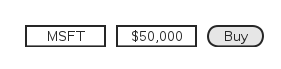
\includegraphics[width=0.300\linewidth]{figures/architecture/buy-form.png}}
\end{figure}

and presses ``Buy''.

In order to process that request, the following must happen:
\setcounter{listcnt0}{0}
\begin{list}{\arabic{listcnt0}.}
{
\usecounter{listcnt0}
\setlength{\rightmargin}{\leftmargin}
}

\item An HTTP post is sent from the browser to the server (Jetty).

\item Jetty delegates the request to the web framework, Lift.

\item Form data is parsed and processed.

\item A call is made to the model to perform the operation.
\end{list}

These steps are described in more detail below.


%___________________________________________________________________________

\paragraph*{\phantomsection%
  4.2.1.2~~~When Lift gets an HTTP POST%
  \addcontentsline{toc}{paragraph}{4.2.1.2~~~When Lift gets an HTTP POST}%
  \label{when-lift-gets-an-http-post}%
}
\begin{figure}
\noindent\makebox[\textwidth][c]{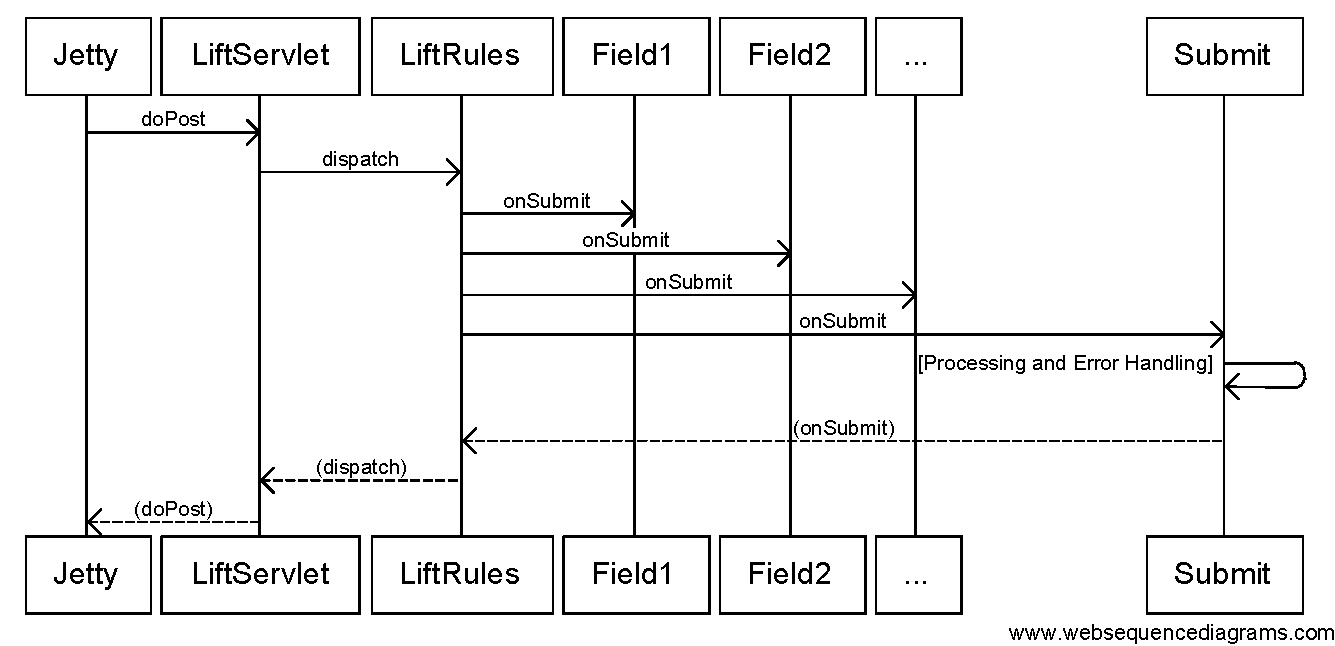
\includegraphics[width=0.900\linewidth]{figures/architecture/form-submission.pdf}}
\end{figure}

PitFail is currently using jQuery to submit forms
(website/html/templates-hidden/default.html ref\_325). Ideally we'd like our
forms to work using either jQuery or traditional HTML forms, but we got this
working first so it's what we're using for now.

When the user hits ``Buy'', JavaScript in the page generates an HTTP POST
directed at PitFail's server. The server Jetty receives the POST, and calls
LiftServlet.doPost() (actually there are some other steps involved because
LiftFilter must first filter the requests but these are all internal to Lift).
LiftServlet passes the request on to LiftRules to dispatch it.

LiftRules recognizes that this is an Ajax request coming from an HTML form, and
extracts the form fields out of it. LiftRules keeps a table of onSubmit
callbacks indexed by field name. For all the incoming fields, Lift calls the
onSubmit callback, and then finally the onSubmit callback for the submit button
-{}- that way, by the time the submit button's callback is invoked, all the
fields will have been invoked first.

We have written a significant amount of code to interface with Lift forms,
which is described in \hyperref[improving-lift-forms]{Improving Lift Forms}.


%___________________________________________________________________________

\paragraph*{\phantomsection%
  4.2.1.3~~~Checking for Consistency%
  \addcontentsline{toc}{paragraph}{4.2.1.3~~~Checking for Consistency}%
  \label{checking-for-consistency}%
}

Scala is a statically typed functional language that has a lot in common with
ML, where the philosphy is that you should use the type system to prove the
consistency of your data at compile-time, eliminating the need for run-time
checks \hyperlink{typing}{[Typing]}.

Unfortunately, this is web programming, where your data is regularly sent to
domains outside of your control. It appears that a strong type system relies a
good deal on trust, which you simply don't have when half your program lives in
a web browser. We found most of our work was spent meticulously pulling
untrusted data back into a strongly typed format, only to have it be clobbered
again at the next page reload.

When a form is submitted, we have to do 2 things with the data:
\setcounter{listcnt0}{0}
\begin{list}{\arabic{listcnt0}.}
{
\usecounter{listcnt0}
\setlength{\rightmargin}{\leftmargin}
}

\item Convert the user's loosely structured input into a strongly-typed internal
representation (example website/view/ModelFields.scala ref\_717).

\item Perform the action requested (example website/view/CommentPage ref\_458).
\end{list}

At either stage something can go wrong.

Because we wrote our own form handling wrappers (\hyperref[improving-lift-forms]{Improving Lift Forms}), we
wrote error handling code for our form wrappers, using a trait called
\texttt{BasicErrors} (website/intform/intform.scala ref\_293). \texttt{BasicErrors} checks
each of the fields in the form for errors; if there are any errors these are
reported to the user, and if all are consistent, it builds a single object
containing all the form data (which is elaborated in \hyperref[improving-lift-forms]{Improving Lift Forms}).

The process of structuring data and checking for input errors looks like this:
\begin{figure}
\noindent\makebox[\textwidth][c]{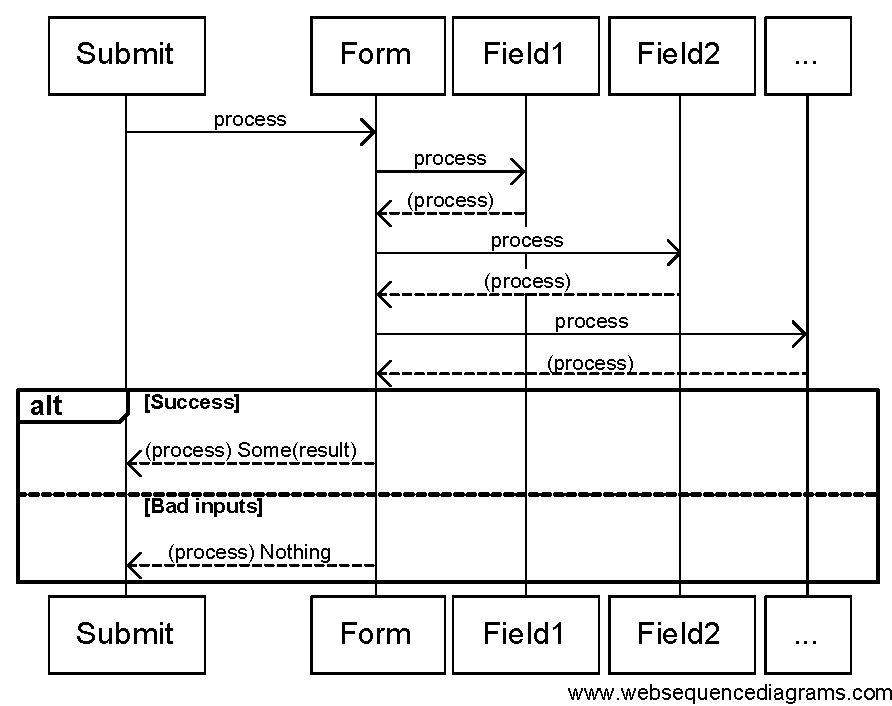
\includegraphics[width=0.900\linewidth]{figures/architecture/input-errors.pdf}}
\end{figure}

If the data makes it past input checking, the operation must be sent to the
domain-specific parts of the code, such as \texttt{Portfolio} or \texttt{StockAsset}.
These operations are described in detail in \hyperref[interactions]{interactions}.

If the operation fails because of something more fundamental -{}- say, for
example, the user attempts to buy more of a stock than is being offered for
sale -{}- the operation will throw an exception (\texttt{NoBidders} in this case)
(model/stocks.scala ref\_478). The View catches the exception and converts it to
a message that will be displayed to the user (example
website/view/StockSeller.scala ref\_736).

We like this system because:
\setcounter{listcnt0}{0}
\begin{list}{\arabic{listcnt0}.}
{
\usecounter{listcnt0}
\setlength{\rightmargin}{\leftmargin}
}

\item The Model (\texttt{Portfolio}, \texttt{StockAsset}, ...) do not have to duplicate the
checks made in the view. For example, the model never needs to check that a
string is formatted correctly like a number.

\item The Model does not have to provide human-readable error mesages; it mearly
throws exceptions, which the View then decides an appropriate message for.
This keeps our code to the MVC pattern.
\end{list}


%___________________________________________________________________________

\section*{\phantomsection%
  5~~~Domain Model%
  \addcontentsline{toc}{section}{5~~~Domain Model}%
  \label{domain-model}%
}


%___________________________________________________________________________

\subsection*{\phantomsection%
  5.1~~~How the Domain Model Has Changed%
  \addcontentsline{toc}{subsection}{5.1~~~How the Domain Model Has Changed}%
  \label{how-the-domain-model-has-changed}%
}

The original domain model diagram looked like this:
\begin{figure}
\noindent\makebox[\textwidth][c]{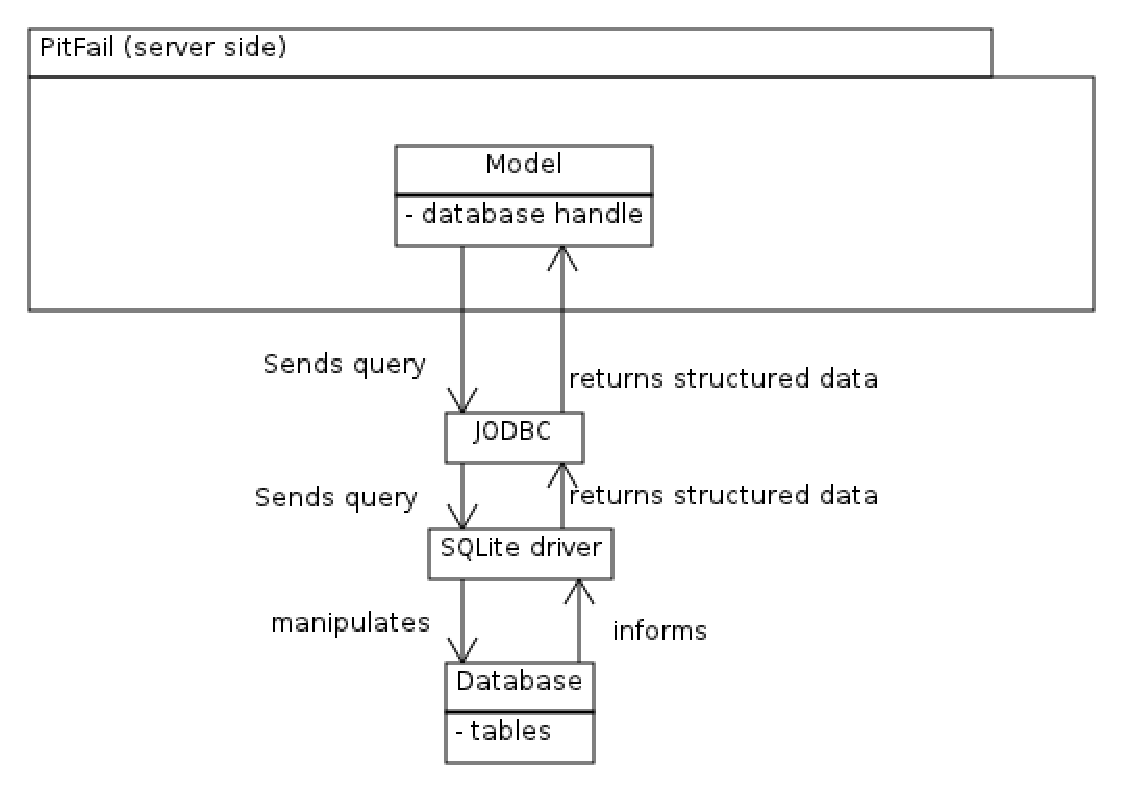
\includegraphics[width=0.900\linewidth]{figures/domain/original-domain.pdf}}
\end{figure}

The single biggest change has been the addition of many more domain specific
concepts to the model. This is mostly due to our improved understanding of the
role that a domain model plays, namely to clarify and define the domain that
the system lives in. The old domain model was much less domain-specific and
more software-specific, which does not serve the original purpose.

The concepts that have been added are domain-specific concepts such as
\texttt{StockAsset}, \texttt{DerivativeAsset}, \texttt{NewsEvent}, \texttt{EventComment}, etc.
(which appear below in the diagrams).

The new domain model has become too complicated to show in a single diagram.
The various pieces of it are diagrammed and explained in the following
sections. What has been \emph{removed} from these sections are architecture-specific
aspects of the system; these have been moved to other sections. The reason is
that the architecture specific parts (how a request comes in, HTTP and AJAX
protocols) are not domain-specific.

One consequence of working more domain concepts into the model is that we had
to include some concepts that do \emph{not} correspond to software objects. This is
noted where it occurs.


%___________________________________________________________________________

\subsection*{\phantomsection%
  5.2~~~Users, Portfolios, and Leagues%
  \addcontentsline{toc}{subsection}{5.2~~~Users, Portfolios, and Leagues}%
  \label{users-portfolios-and-leagues}%
}


%___________________________________________________________________________

\subsubsection*{\phantomsection%
  5.2.1~~~Basic Definitions%
  \addcontentsline{toc}{subsubsection}{5.2.1~~~Basic Definitions}%
  \label{basic-definitions}%
}
%
\begin{itemize}

\item ``User'' -{}- A human player of PitFail. A user may manage more than one
portfolio.

\item ``Portfolio'', aka ``Team'' aka ``Company'' -{}- A made-up PitFail entity that \emph{owns}
and \emph{trades}. Many times in this document it may be mentioned that a
``portfolio'' places an order. The reason for this phrasing is that the order
is associated with a portfolio, not with a user. The primary traders in
PitFail are portfolios. A portfolio may be owned by more than one user.

\item ``League'' -{}- a collection of portfolios competing against each other. A league
is managed by a User, but participated in by Portfolios. Hence a single user
may have portfolios that belong to different leagues.

\end{itemize}

An example might help to illustrate what is going on here:
\begin{figure}
\noindent\makebox[\textwidth][c]{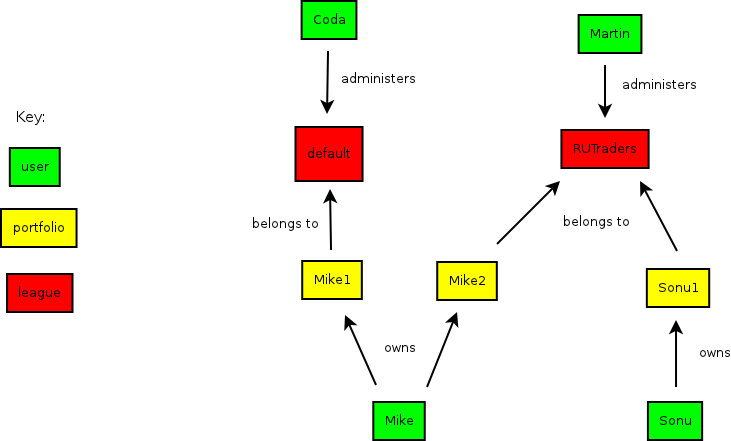
\includegraphics[width=0.900\linewidth]{figures/domain/user-example.png}}
\end{figure}

In this example, Mike and Sonu are users. Mike has two portfolios, named Mike1
and Mike2; Sonu has 1 portfolio, named Sonu1. Mike1 belongs to a league named
``default''; Mike2 and Sonu1 belong to a league named ``RUTraders''.

Coda and Martin are users that administer the ``default'' and ``RUTraders''
leagues. Coda and Martin might have portfolios of their own, but this is not
relevant to the business of administering leagues.

The reasons for the existence of each of these concepts is:
%
\begin{itemize}

\item ``User'' -{}- This provides a way for an actual human user to log into the site,
to have an experience that is tied to them.

\item ``Portfolio'' -{}- These actually do the trading. A Portfolio is the one actually
credited with owning assets and being responsible for the payment of
liabilities, \emph{not} the user.

\item ``League'' -{}- The purpose of a league is to represent ``competition'' between
portfolios. Hence rankings are done within a league, and ``rules'' are set
within a league. Trading, however, happens globally, among all leagues.

\end{itemize}

In the report we will often say that ``a portfolio does this'' and ``a portfolio
does that''; the action is being initiated by a human, but we model it as if the
portfolio is the doer of an action: a portfolio buys a stock, a portfolio sells
a stock. If we want to refer to a real human being we will use the word
``player''.


%___________________________________________________________________________

\subsubsection*{\phantomsection%
  5.2.2~~~The User-Portfolio-League domain model%
  \addcontentsline{toc}{subsubsection}{5.2.2~~~The User-Portfolio-League domain model}%
  \label{the-user-portfolio-league-domain-model}%
}

The basic concepts and relationships for the idle system are:
\begin{figure}
\noindent\makebox[\textwidth][c]{
\includegraphics[width=0.900\linewidth]{figures/domain/users.png}}
\end{figure}

Adding some of the creation/joining operations, this becomes:
\begin{figure}
\noindent\makebox[\textwidth][c]{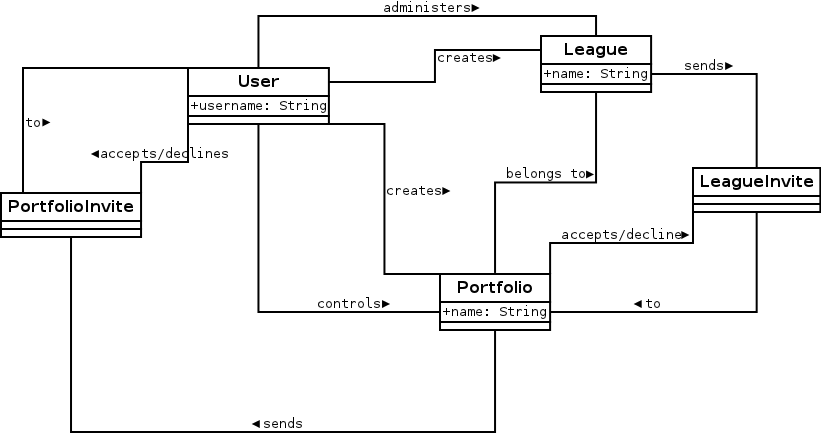
\includegraphics[width=0.900\linewidth]{figures/domain/users2.png}}
\end{figure}

Note a few potentially surprising things about this model:
%
\begin{itemize}

\item PortfolioInvites are sent to Users, and LeagueInvites are sent to Portfolios.
This is because it is a User who will control a portfolio, and a Portfolio
that will join a league (users do not join leagues).

\item Even though, in reality, a human user initiates the action of ``sending'' an
invite, it is shown in the diagram as originating from a Portfolio or a
League, because that is how we interpret it; invites  come from the concepts
that can be joined.

\end{itemize}

In the actual code, some of the ``many-to-many'' relationships acquired an extra
class (the association class). Such as (model/users.scala):
\begin{figure}
\noindent\makebox[\textwidth][c]{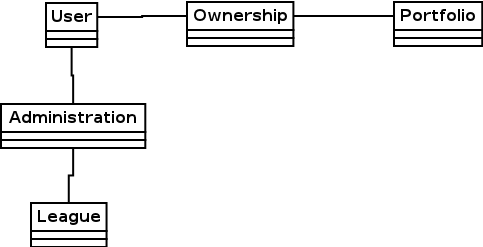
\includegraphics[width=0.900\linewidth]{figures/domain/association.png}}
\end{figure}

But this is a detail of the implementation and not part of the domain model; no
meaningful attributes are stored with Ownership and Administration.


%___________________________________________________________________________

\subsection*{\phantomsection%
  5.3~~~Assets and Liabilities%
  \addcontentsline{toc}{subsection}{5.3~~~Assets and Liabilities}%
  \label{assets-and-liabilities}%
}

This part describes only the \emph{ownership} aspect of assets and liabilities. The
trading and exercising aspects will be described later.

The diagram below shows only the part of the domain model that relate to the
ownership of assets and liabilities:
\begin{figure}
\noindent\makebox[\textwidth][c]{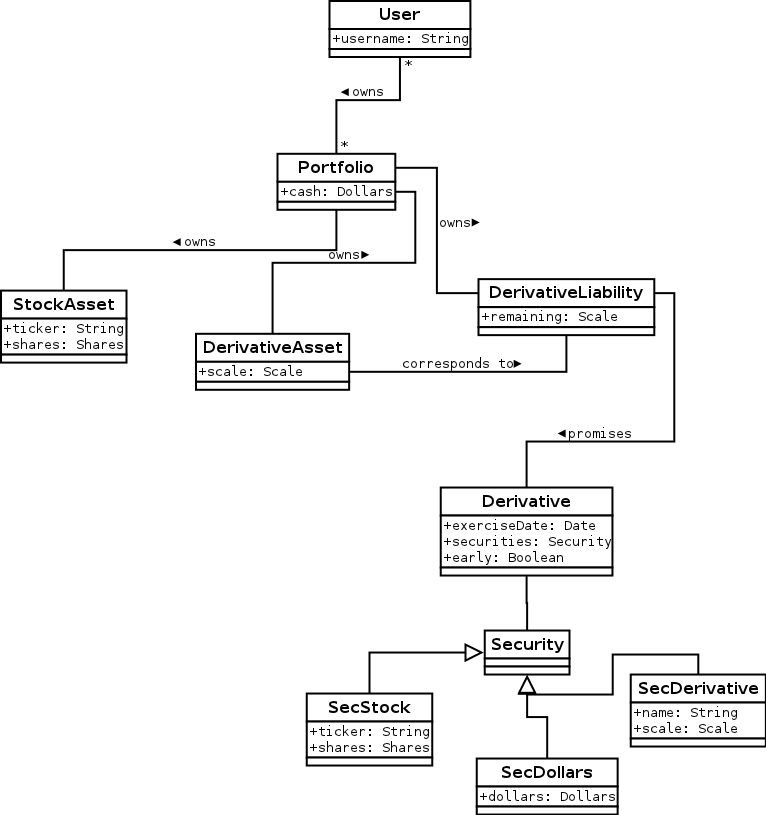
\includegraphics[width=0.900\linewidth]{figures/domain/assets.png}}
\end{figure}

There are two kinds of assets: StockAssets and DerivativeAssets, and one kind
of liability: a DerivativeLiability.


%___________________________________________________________________________

\subsubsection*{\phantomsection%
  5.3.1~~~How StockAssets work%
  \addcontentsline{toc}{subsubsection}{5.3.1~~~How StockAssets work}%
  \label{how-stockassets-work}%
}

A stock asset is simply a number of shares of a particular stock. So for
example, 30 shares of MSFT is a stock asset.


%___________________________________________________________________________

\subsubsection*{\phantomsection%
  5.3.2~~~How Derivative Assets/Liabilities work%
  \addcontentsline{toc}{subsubsection}{5.3.2~~~How Derivative Assets/Liabilities work}%
  \label{how-derivative-assets-liabilities-work}%
}

A derivative, in PitFail, is a promise to exchange a list of assets on or
before a specified date. There are 3 parts to this contract:
\setcounter{listcnt0}{0}
\begin{list}{\arabic{listcnt0}.}
{
\usecounter{listcnt0}
\setlength{\rightmargin}{\leftmargin}
}

\item The \emph{Derivative} is the statement of the contract; that is, it is the list
of assets to be exchanged, the date on which it is to occur, and whether the
contract may be exercised early (See for example \hyperlink{american}{[American]}). The exact
nature of how the contract is specified is described in the section on
\hyperref[derivativeexp]{derivativeexp}.

\item The \emph{DerivativeLiability} is the statement by one portfolio that they will
offer up the assets specified in the Derivative.

\item The \emph{DerivativeAsset} is a promise to a portfolio that they will be able to collect
the assets promised in the Derivative.
\end{list}

Each DerivativeAsset corresponds to exactly 1 DerivativeLiability, and each
DerivativeLiability corresponds to 1 or more DerivativeAssets. Each
DerivativeAsset has a property called \texttt{scale} which is the portion of the
liability this asset has a claim on. A DerivativeLiability has an attribute
\texttt{remaining} which is the fraction of the contract that has \emph{not} been
exercised:
\begin{figure}
\noindent\makebox[\textwidth][c]{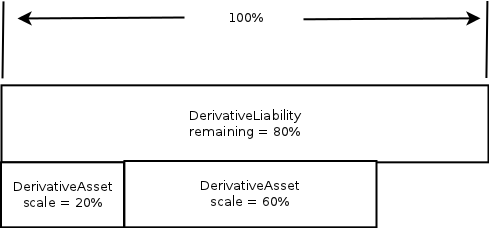
\includegraphics[width=0.900\linewidth]{figures/domain/scale.png}}
\end{figure}

Every time a DerivativeAsset is exercised, it is deleted, and the \texttt{remaining}
of the corresponding DerivativeLiability is reduced by the \texttt{scale} of the
DerivativeAsset. It is an invariant of the system that the sum of of the scales
of all DerivativeAssets for a particular DerivativeLiability must equal the
\texttt{remaining}.


%___________________________________________________________________________

\subsection*{\phantomsection%
  5.4~~~Derivatives%
  \addcontentsline{toc}{subsection}{5.4~~~Derivatives}%
  \label{derivatives}%
  \label{derivativeexp}%
}

The parts to a derivative contract are:
\setcounter{listcnt0}{0}
\begin{list}{\arabic{listcnt0}.}
{
\usecounter{listcnt0}
\setlength{\rightmargin}{\leftmargin}
}

\item A list of securities to be traded.

\item A date on which this is to occur.

\item Whether it may be exercised early.

\item A condition that decides (automatically) whether the derivative will be
exercised on the scheduled date.
\end{list}

(2) and (3) are just a \texttt{DateTime} and a \texttt{Boolean} respectively; (1) is
more complicated.

The list of securities is represented as a list, where each element may be one
of:
\setcounter{listcnt0}{0}
\begin{list}{\arabic{listcnt0}.}
{
\usecounter{listcnt0}
\setlength{\rightmargin}{\leftmargin}
}

\item A ``stock'' security, \texttt{SecStock}, which holds a ticker symbol and a number
of shares.

\item A ``dollars'' security, \texttt{SecDollar}, which holds a dollar amount.

\item A ``derivative'' security, \texttt{SecDerivative}, which holds a named liability
and a scale (see the section on \hyperref[scaling-derivatives]{Scaling Derivatives}). (At the moment
there is no way within the PitFail UI to create a \texttt{SecDerivative}.
However, since the theoretical concepts behind it are complete, we describe
it anyway).
\end{list}

If any of the quantities are negative (eg negative shares, negative dollars,
negative scale), that means that the securities are supposed to move from the
buyer to the seller.

For a descripton of how derivatives are exercised see \hyperref[exercising-derivatives]{Exercising
Derivatives}.


%___________________________________________________________________________

\subsubsection*{\phantomsection%
  5.4.1~~~Scaling Derivatives%
  \addcontentsline{toc}{subsubsection}{5.4.1~~~Scaling Derivatives}%
  \label{scaling-derivatives}%
}

Many aspects of PitFail require that derivatives be scaled. That is, given one
derivative, create a new one with identical terms, but ``smaller'' or ``larger'':
\begin{figure}
\noindent\makebox[\textwidth][c]{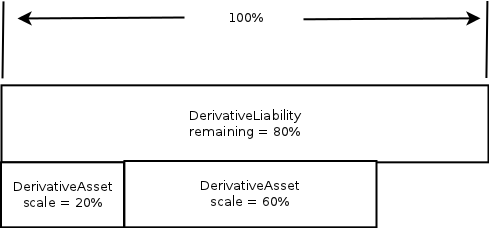
\includegraphics[width=0.900\linewidth]{figures/domain/scale.png}}
\end{figure}

Scaling is done by scaling each security promised:
\setcounter{listcnt0}{0}
\begin{list}{\arabic{listcnt0}.}
{
\usecounter{listcnt0}
\setlength{\rightmargin}{\leftmargin}
}

\item For SecDollar, scale the dollar amount

\item For SecStock, scale the share amount

\item For SecDerivative, scale the scale amount
\end{list}

and leaving the date and early exercise the same.


%___________________________________________________________________________

\subsection*{\phantomsection%
  5.5~~~Trading Stocks%
  \addcontentsline{toc}{subsection}{5.5~~~Trading Stocks}%
  \label{trading-stocks}%
}

The diagram below represents the ``idle state'' of the system with respect to
stock trading:
\begin{figure}
\noindent\makebox[\textwidth][c]{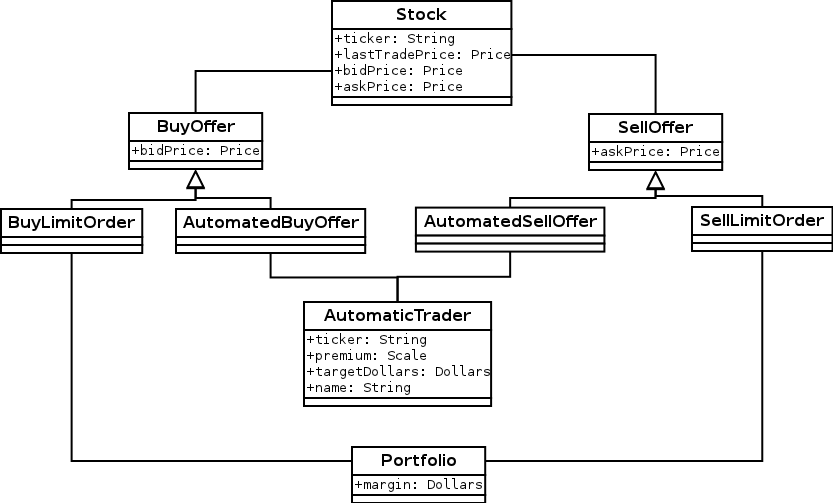
\includegraphics[width=0.900\linewidth]{figures/domain/trading.png}}
\end{figure}

When the system is is idle, no trades are taking place; all that exist are
orders that have yet to be fulfilled.

PitFail allows only two kinds of orders to sit idly. These are
\setcounter{listcnt0}{0}
\begin{list}{\arabic{listcnt0}.}
{
\usecounter{listcnt0}
\setlength{\rightmargin}{\leftmargin}
}

\item Limit orders

\item Autamated (synthetic) trading orders.
\end{list}

Market orders do not exist when the system is idle because market orders are
executed at the offering price as soon as they are created. PitFail does not
provide explicit support for stop orders, but it would be easy for a user to
create one using the javascript automated trading API (and, when a Stop is
triggered, it becomes a market order \hyperlink{stop}{[Stop]}, and so will be executed
immediately).

All orders in the idle state have two important properties: the available
number of shares, and the limit price. This will allow PitFail to form
automatic matches, as described later.

An invariant of the system is that when the order system is Idle, there are no
orders that can be matched with one another.


%___________________________________________________________________________

\subsubsection*{\phantomsection%
  5.5.1~~~When a new order comes in%
  \addcontentsline{toc}{subsubsection}{5.5.1~~~When a new order comes in}%
  \label{when-a-new-order-comes-in}%
}

When a new order comes in, it has a desired number of shares, and it may or may
not have a limit price. First, all existing orders for the same stock are
collected, and sorted by desirability (ie, best price to worst price):
\begin{figure}
\noindent\makebox[\textwidth][c]{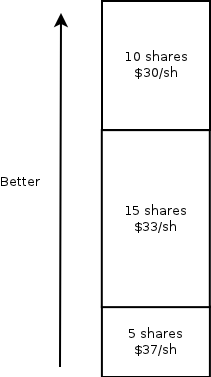
\includegraphics[width=0.900\linewidth]{figures/domain/available1.png}}
\end{figure}

The incoming order is matched up against the best orders possible (that are
below its limit price, if any). Those orders are then completely or partially
executed:
\begin{figure}
\noindent\makebox[\textwidth][c]{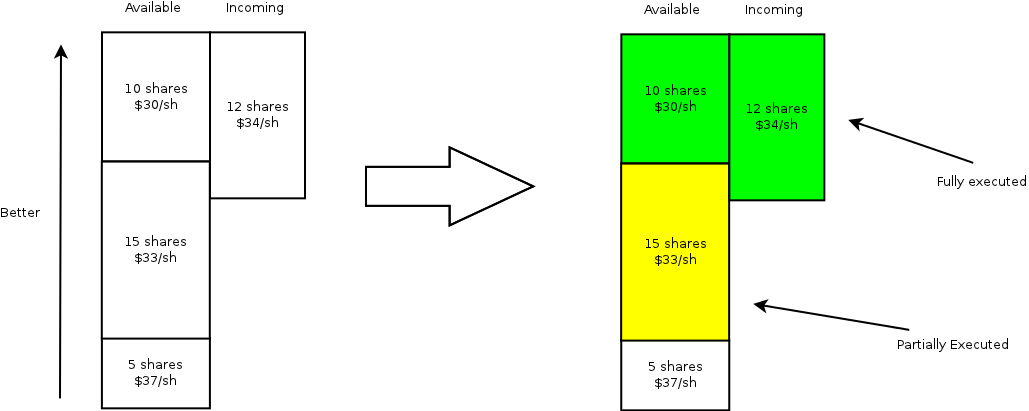
\includegraphics[width=0.900\linewidth]{figures/domain/execution.png}}
\end{figure}

In this example, 10 shares will be purchased at 30/sh, and 2 shares at 33/sh.

You will notice that the orders already \emph{in} the pool pay a price in not being
able to negotiate -{}- since the buyer is willing to pay 34/sh, they would, if
they could, increase their limit to 34/sh to take advantage. However, by having
orders in the pool that are \emph{not} negotiated, there is a benefit in liquidity;
hence traders who place orders unexecuted into the pool will change a liquidity
premium in the trade (which is why there is a spread between the bid and ask
price for a stock as offered by the same trader \hyperlink{makers}{[Makers]}).

If the newly placed order is not fully executed, and the trader specified a
limit, it will become part of the pool of unexecuted orders.


%___________________________________________________________________________

\subsubsection*{\phantomsection%
  5.5.2~~~Margin%
  \addcontentsline{toc}{subsubsection}{5.5.2~~~Margin}%
  \label{margin}%
}

In order to ensure the smooth execution of orders, when a user places an order
that is not executed immediately, they must set aside margin so that the order
can be executed later. For a buy order the user sets aside cash that will be
used to buy the shares when the order is executed, and for a sell order the
user sets aside the shares that will be sold.

If the order is cancelled or not fully used the margin will be returned.


%___________________________________________________________________________

\subsubsection*{\phantomsection%
  5.5.3~~~Domain model for trading%
  \addcontentsline{toc}{subsubsection}{5.5.3~~~Domain model for trading}%
  \label{domain-model-for-trading}%
}

The model below does not correspond 1-1 to actual software classes because our
architecture is not entirely object-oriented. For example, there is no class
called Execution; execution of orders is procedural.
\begin{figure}
\noindent\makebox[\textwidth][c]{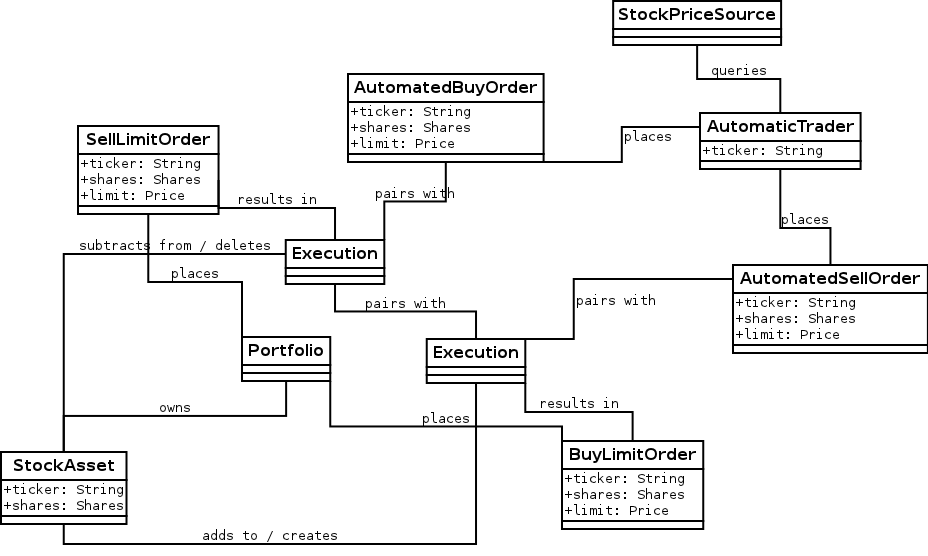
\includegraphics[width=0.900\linewidth]{figures/domain/trading2.png}}
\end{figure}

The association of AutomaticTrader with StockPriceSource is meant to convey
that the automatic traders use real-world bid and ask prices to set their bid
and ask prices.

Because there is too much to fit on one diagram, here is the part of the domain
model that deals with cash and margin:
\begin{figure}
\noindent\makebox[\textwidth][c]{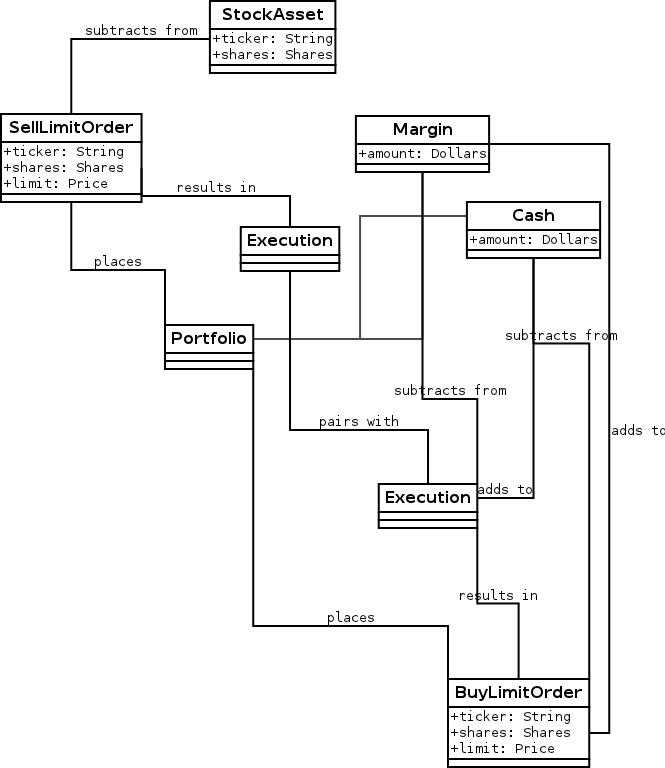
\includegraphics[width=0.900\linewidth]{figures/domain/trading3.png}}
\end{figure}

(In the code, there is no object called Cash, rather it is an attribute of
Portfloio; but it is helpful to show it as such for the domain model).

The reason that the execution of a BuyLimitOrder ``adds to'' Cash is that all the
necessary cash has already been set aside in Margin; the cash that is being
added is the leftover margin.

When an order is cancelled (by its owner), all that must happen is that the
margin is restored:
\begin{figure}
\noindent\makebox[\textwidth][c]{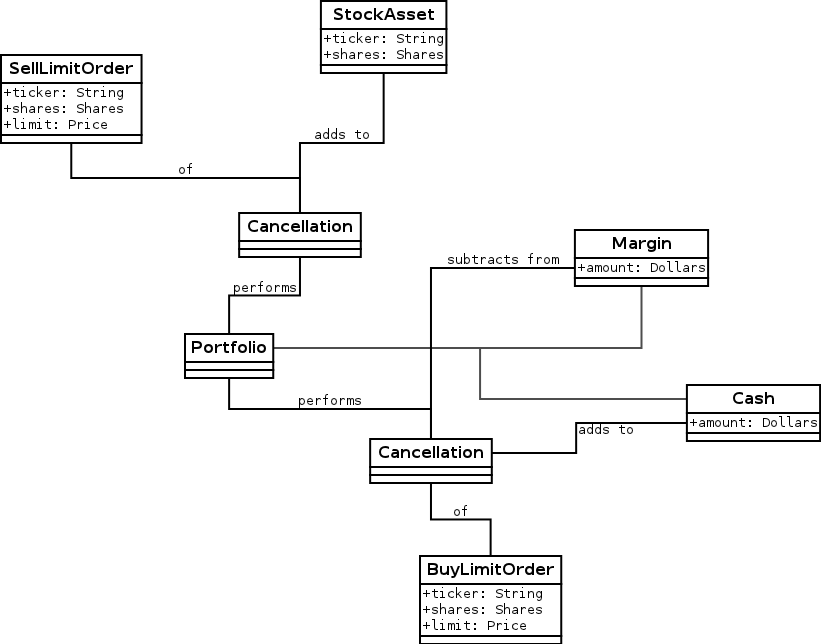
\includegraphics[width=0.900\linewidth]{figures/domain/trading4.png}}
\end{figure}


%___________________________________________________________________________

\subsection*{\phantomsection%
  5.6~~~Dividends%
  \addcontentsline{toc}{subsection}{5.6~~~Dividends}%
  \label{dividends}%
}

It is very important for PitFail to keep track of dividends paid by stocks,
for two reasons:
\setcounter{listcnt0}{0}
\begin{list}{\arabic{listcnt0}.}
{
\usecounter{listcnt0}
\setlength{\rightmargin}{\leftmargin}
}

\item It would be unrealistic in a particularly unsettling way: stocks that will
never pay dividends have no value; why are we trading them?

\item Because PitFail players will own stocks that pay dividends, and every time a
dividend is paid the stock price drops abruptly, players would not
appreciate having the price drop if they do not receive a dividend in
return.
\end{list}

Periodically, PitFail queries Yahoo Finance to see if stocks owned by the
players have paid dividends. If they have, the system will pay dividends to the
player, in what is represented here (though not in the code) as a
\texttt{DividendEvent}:
\begin{figure}
\noindent\makebox[\textwidth][c]{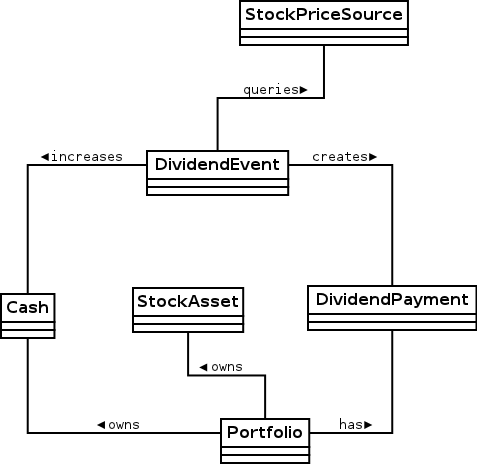
\includegraphics[width=0.900\linewidth]{figures/domain/dividends1.png}}
\end{figure}

The \texttt{DividendPayment} object is created only to allow the user to view the
history of their dividend payments.


%___________________________________________________________________________

\subsection*{\phantomsection%
  5.7~~~News%
  \addcontentsline{toc}{subsection}{5.7~~~News}%
  \label{news}%
}

The purpose of ``news'' is to show PitFail players to see what other PitFail
players have been doing. Importantly, News is not part of actual trading; this
is just for seeing what's going on.

This means that a single news event has associations with a lot of other
concepts, but not in a way that affects the rest of the program: it's just
point out, for example, which derivative was traded when reporting that a
derivative was traded.

The basic model for News is:
\begin{figure}
\noindent\makebox[\textwidth][c]{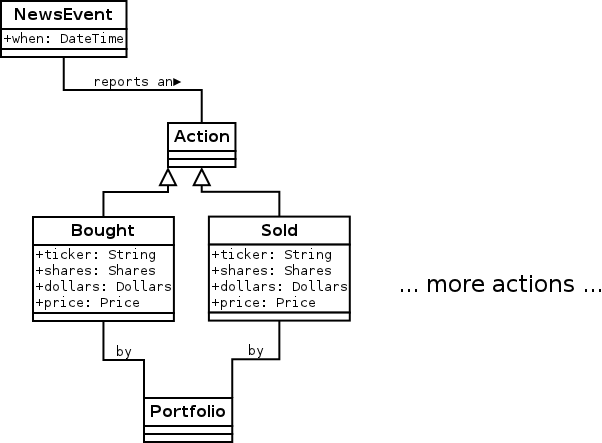
\includegraphics[width=0.900\linewidth]{figures/domain/news1.png}}
\end{figure}

only two actions are shown here; there are a lot so they are split up across
multiple diagrams.

Buying and selling stocks, as shown above, refer to the Portfolio who ``did'' the
action, and the information about what was bought or sold. This only applies to
orders that are executed (either immediately or later). Orders that are delayed
will generate another kind of an event.

Derivative Trading has the following kinds of events:
\begin{figure}
\noindent\makebox[\textwidth][c]{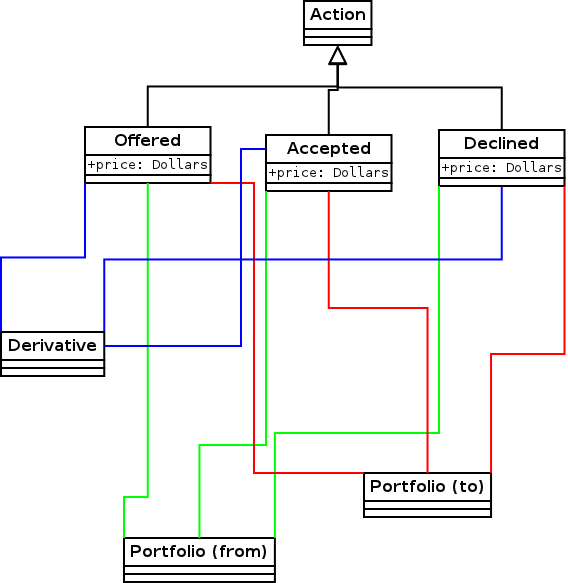
\includegraphics[width=0.900\linewidth]{figures/domain/news2.png}}
\end{figure}

\texttt{from} and \texttt{to} are shown as separate concepts even though they are
instances of the same class, because they play a different role in these
events: one is the portfolio making the offer, the other is the portfolio
receiving, and possible accepting, the offer.

For Auctions we have:
\begin{figure}
\noindent\makebox[\textwidth][c]{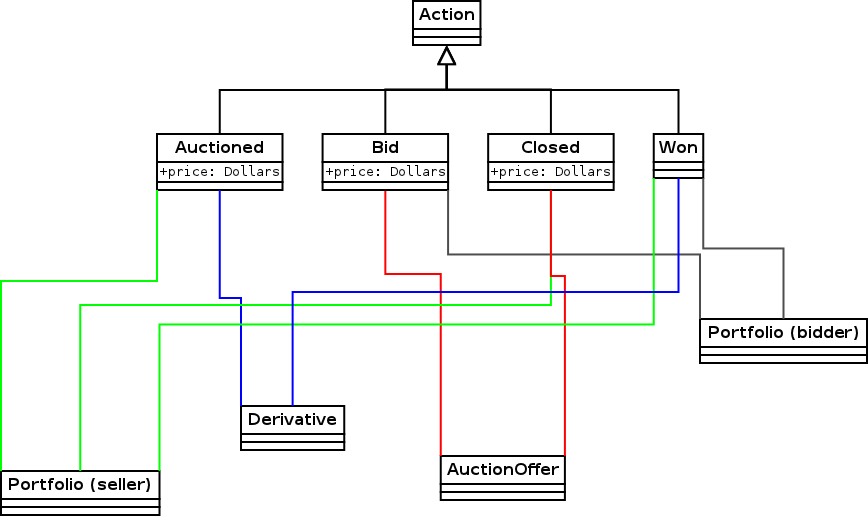
\includegraphics[width=0.900\linewidth]{figures/domain/news3.png}}
\end{figure}

There are other associations which are not shown, that relate to voting. These
are described in the section on voting.

Placing orders that get delayed are described by:
\begin{figure}
\noindent\makebox[\textwidth][c]{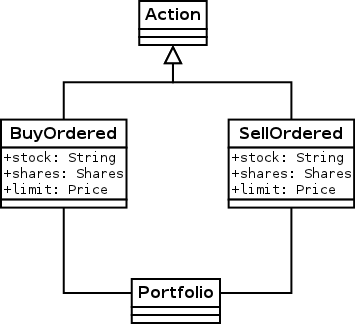
\includegraphics[width=0.900\linewidth]{figures/domain/news4.png}}
\end{figure}

Where the associated portfolio is the one who performed the buy or sell.

There is one more event for exercising derivatives:

% .. figure:: news5.png

Where the associated portfolio is the one who did the exercising.


%___________________________________________________________________________

\subsection*{\phantomsection%
  5.8~~~Voting%
  \addcontentsline{toc}{subsection}{5.8~~~Voting}%
  \label{voting}%
}

When players enter into a contract involving a derivative, the following assets
are moved:
\begin{figure}
\noindent\makebox[\textwidth][c]{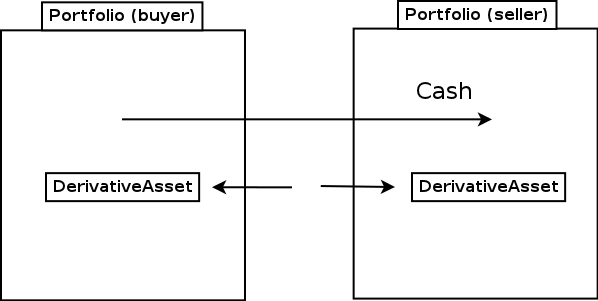
\includegraphics[width=0.900\linewidth]{figures/domain/voting1.png}}
\end{figure}

If owning the asset (being in the buyer side of the contract) pays off more
than the cash payed, the buyer is happy. If owning the liability (being in the
seller side of the contract) is not bad enough to negate the cash received, the
seller got a good deal. These are not necessarily mutually exclusive.

Now, say a third player, the Voter, looks at his news feed and thinks that the
buyer got a good deal (and maybe the seller too, but that is not relevant yet).
The Voter would be happy with an arrangement like the following:
\begin{figure}
\noindent\makebox[\textwidth][c]{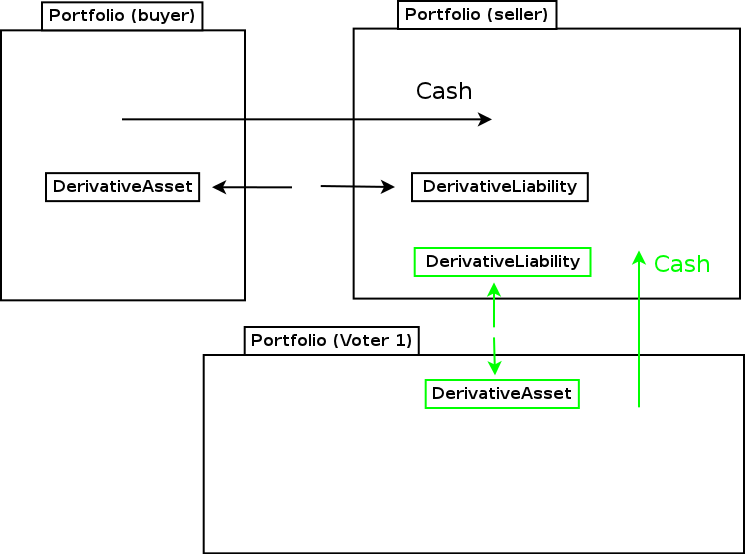
\includegraphics[width=0.900\linewidth]{figures/domain/voting2.png}}
\end{figure}

where the derivative in green resembles the derivative in black, and the cash
in green resembles the cash in black. (As in, if it was a good deal for him,
it's a good deal for me too. Not necessarily true, but it could be true
sometimes).

When two portfolios enter a derivative, an object is created called
\texttt{DerivativeBuyerSetAside} (there is a nearly identical process for sellers,
which is discussed next):
\begin{figure}
\noindent\makebox[\textwidth][c]{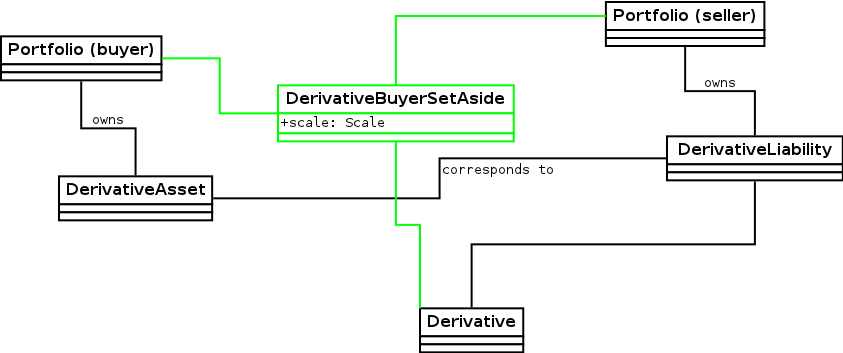
\includegraphics[width=0.900\linewidth]{figures/domain/voting3.png}}
\end{figure}

(remember, the Derivative holds the terms of the contract, and the
DerivativeAsset and DerivativeLiability show who owns which end).

The DerivativeBuyerSetAside holds one attribute, which is the ``amount'' left to
be voted on. For the precise meaning of this scale, see the section on \hyperref[scaling-derivatives]{Scaling
Derivatives}.

The \texttt{scale} remaining starts out at 3\%. When the first voter votes in favor
of the buyer, they enter into a contract with the seller that is identical to
the original derivative, but scaled to 1.5\% (= 3\%/2). He also pays the seller
1.5\% of what the original buyer paid:
\begin{figure}
\noindent\makebox[\textwidth][c]{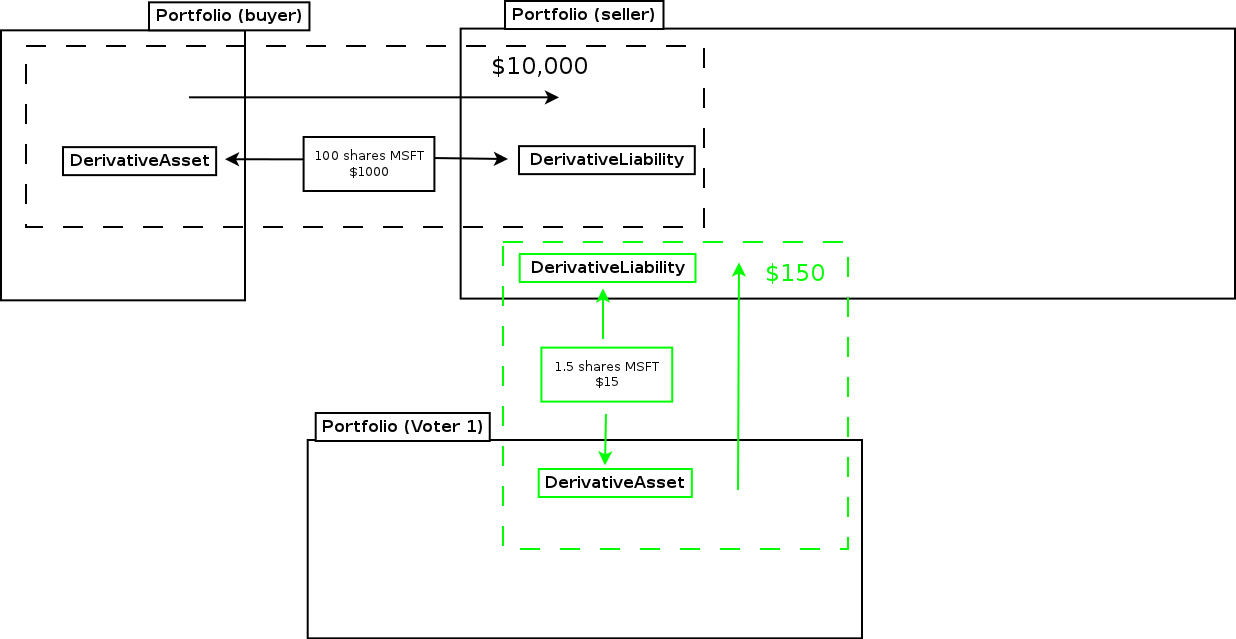
\includegraphics[width=0.900\linewidth]{figures/domain/voting4.png}}
\end{figure}

The \texttt{scale} remaining is then cut by half to 1.5\%.

Now if another player votes, they will realize 0.75\% of the original trade:
\begin{figure}
\noindent\makebox[\textwidth][c]{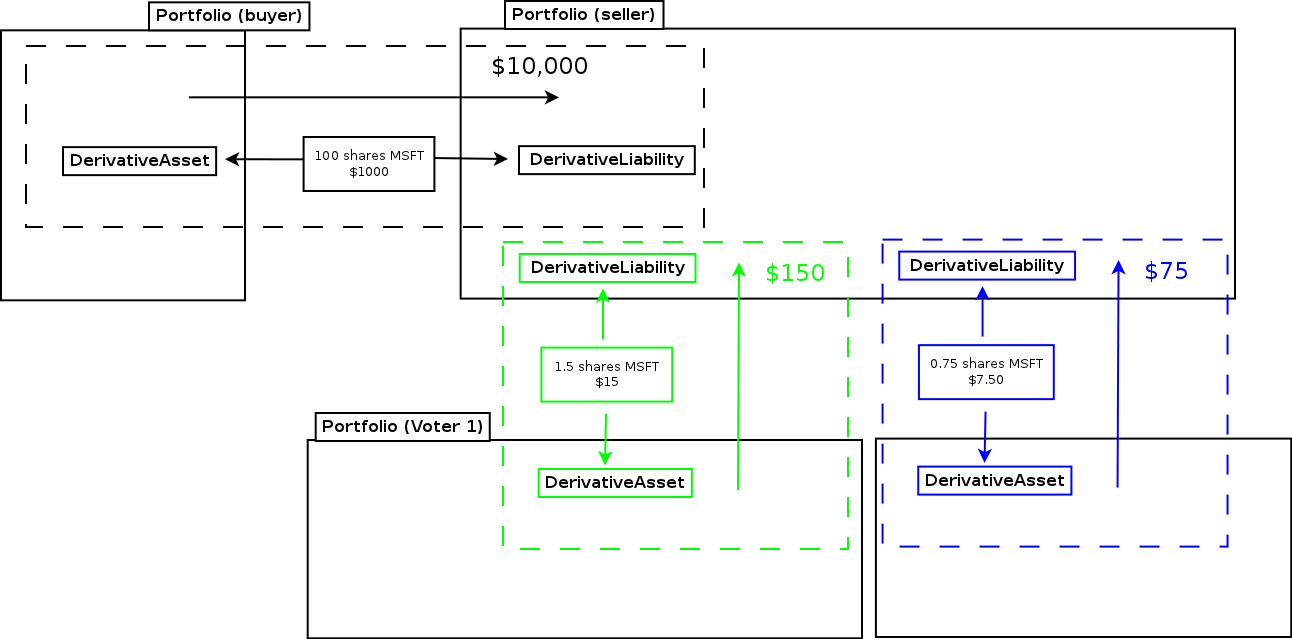
\includegraphics[width=0.900\linewidth]{figures/domain/voting5.png}}
\end{figure}

Votes are recorded and associated with the origanal NewsEvent, so that a score
of buyer-votes and seller votes can be calculated:
\begin{figure}
\noindent\makebox[\textwidth][c]{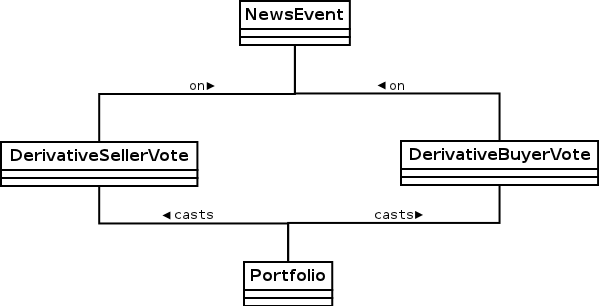
\includegraphics[width=0.900\linewidth]{figures/domain/voting6.png}}
\end{figure}


%___________________________________________________________________________

\subsection*{\phantomsection%
  5.9~~~Comments%
  \addcontentsline{toc}{subsection}{5.9~~~Comments}%
  \label{comments}%
}

Compared to voting, comments are refreshingly simple.

Users, not portfolios, cast comments. A comment is associated with a news
event:
\begin{figure}
\noindent\makebox[\textwidth][c]{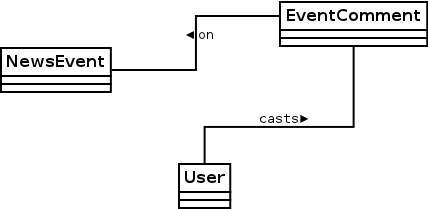
\includegraphics[width=0.900\linewidth]{figures/domain/comments1.png}}
\end{figure}


%___________________________________________________________________________

\subsection*{\phantomsection%
  5.10~~~Auto Trades%
  \addcontentsline{toc}{subsection}{5.10~~~Auto Trades}%
  \label{auto-trades}%
}

While the system is idle, an auto-trade is represented as:
\begin{figure}
\noindent\makebox[\textwidth][c]{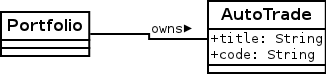
\includegraphics[width=0.900\linewidth]{figures/domain/auto1.png}}
\end{figure}

When a player runs an AutoTrade, we have what we conceptually (though not in
the code) call an AutoTradeEvent:
\begin{figure}
\noindent\makebox[\textwidth][c]{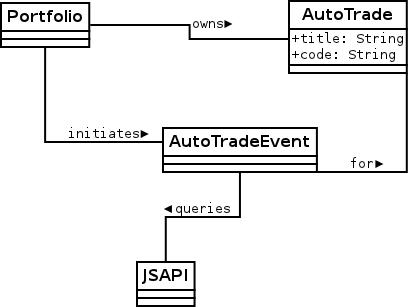
\includegraphics[width=0.900\linewidth]{figures/domain/auto2.png}}
\end{figure}

The \texttt{JSAPI} is a set of JavaScript functions and corresponding server-side
handlers that allow the Auto Trade to actually perform actions.


%___________________________________________________________________________

\section*{\phantomsection%
  6~~~Perturbations and Interactions%
  \addcontentsline{toc}{section}{6~~~Perturbations and Interactions}%
  \label{perturbations-and-interactions}%
}


%___________________________________________________________________________

\subsection*{\phantomsection%
  6.1~~~Stocks%
  \addcontentsline{toc}{subsection}{6.1~~~Stocks}%
  \label{stocks}%
  \label{interactions}%
}


%___________________________________________________________________________

\subsubsection*{\phantomsection%
  6.1.1~~~\texttt{allStockHoldings}%
  \addcontentsline{toc}{subsubsection}{6.1.1~~~allStockHoldings}%
  \label{allstockholdings}%
}

Gets all stocks held in PitFail (model/stocks.scala ref\_158).
\begin{figure}
\noindent\makebox[\textwidth][c]{\includegraphics[width=0.900\linewidth]{figures/interactions/allStockHoldings.pdf}}
\end{figure}


%___________________________________________________________________________

\subsubsection*{\phantomsection%
  6.1.2~~~\texttt{Portfolio.myStockAssets}%
  \addcontentsline{toc}{subsubsection}{6.1.2~~~Portfolio.myStockAssets}%
  \label{portfolio-mystockassets}%
}

Gets stock assets from this portfolio (model/stocks.scala ref\_937).
\begin{figure}
\noindent\makebox[\textwidth][c]{\includegraphics[width=0.900\linewidth]{figures/interactions/myStockAssets.pdf}}
\end{figure}


%___________________________________________________________________________

\subsubsection*{\phantomsection%
  6.1.3~~~\texttt{Portfolio.haveTicker}%
  \addcontentsline{toc}{subsubsection}{6.1.3~~~Portfolio.haveTicker}%
  \label{portfolio-haveticker}%
}

Gets an asset for this stock if we have one, None otherwise (model/stocks.scala ref\_407).
\begin{figure}
\noindent\makebox[\textwidth][c]{\includegraphics[width=0.900\linewidth]{figures/interactions/haveTicker.pdf}}
\end{figure}


%___________________________________________________________________________

\subsubsection*{\phantomsection%
  6.1.4~~~\texttt{Portfolio.howManyShares}%
  \addcontentsline{toc}{subsubsection}{6.1.4~~~Portfolio.howManyShares}%
  \label{portfolio-howmanyshares}%
}

Gets how many shares of this stock do we have (model/stocks.scala ref\_666).
\begin{figure}
\noindent\makebox[\textwidth][c]{\includegraphics[width=0.900\linewidth]{figures/interactions/howManyShares.pdf}}
\end{figure}


%___________________________________________________________________________

\subsubsection*{\phantomsection%
  6.1.5~~~\texttt{Portfolio.howManyDollars}%
  \addcontentsline{toc}{subsubsection}{6.1.5~~~Portfolio.howManyDollars}%
  \label{portfolio-howmanydollars}%
}

Gets how many dollars (at last traded price) of this stock we have
(model/stocks.scala ref\_873).
\begin{figure}
\noindent\makebox[\textwidth][c]{\includegraphics[width=0.900\linewidth]{figures/interactions/howManyDollars.pdf}}
\end{figure}


%___________________________________________________________________________

\subsubsection*{\phantomsection%
  6.1.6~~~\texttt{Portfolio.userBuyStock}%
  \addcontentsline{toc}{subsubsection}{6.1.6~~~Portfolio.userBuyStock}%
  \label{portfolio-userbuystock}%
}

Attempts to make a market-order purchase of a stock (model/stocks.scala
ref\_850).
\begin{figure}
\noindent\makebox[\textwidth][c]{\includegraphics[width=0.900\linewidth]{figures/interactions/userBuyStock.pdf}}
\end{figure}


%___________________________________________________________________________

\subsubsection*{\phantomsection%
  6.1.7~~~\texttt{Portfolio.userSellStock}%
  \addcontentsline{toc}{subsubsection}{6.1.7~~~Portfolio.userSellStock}%
  \label{portfolio-usersellstock}%
}

Makes a sell market order for a stock (model/stocks.scala ref\_620).
\begin{figure}
\noindent\makebox[\textwidth][c]{\includegraphics[width=0.900\linewidth]{figures/interactions/userSellStock.pdf}}
\end{figure}


%___________________________________________________________________________

\subsubsection*{\phantomsection%
  6.1.8~~~\texttt{Portfolio.userSellAll}%
  \addcontentsline{toc}{subsubsection}{6.1.8~~~Portfolio.userSellAll}%
  \label{portfolio-usersellall}%
}

Sells all of the shares we own (with a market order)(model/stocks.scala
ref\_306).
\begin{figure}
\noindent\makebox[\textwidth][c]{\includegraphics[width=0.900\linewidth]{figures/interactions/userSellAll.pdf}}
\end{figure}


%___________________________________________________________________________

\subsubsection*{\phantomsection%
  6.1.9~~~\texttt{Portfolio.userMakeBuyLimitOrder}%
  \addcontentsline{toc}{subsubsection}{6.1.9~~~Portfolio.userMakeBuyLimitOrder}%
  \label{portfolio-usermakebuylimitorder}%
}

Places a buy limit order. This involves first executing all of the order that
can be executed immediately (ie there are available sellers below the limit)
and then deferring the rest until another available seller comes in
(model/stocks.scala ref\_184).
\begin{figure}
\noindent\makebox[\textwidth][c]{\includegraphics[width=0.900\linewidth]{figures/interactions/userMakeBuyLimitOrder.pdf}}
\end{figure}


%___________________________________________________________________________

\subsubsection*{\phantomsection%
  6.1.10~~~\texttt{Portfolio.userMakeSellLimitOrder}%
  \addcontentsline{toc}{subsubsection}{6.1.10~~~Portfolio.userMakeSellLimitOrder}%
  \label{portfolio-usermakeselllimitorder}%
}

Places a sell limit order. This involves executing all that can be executed
immediately (where ther are available buyers above the limit) and then defers
the rest (model/stocks.scala ref\_939).
\begin{figure}
\noindent\makebox[\textwidth][c]{\includegraphics[width=0.900\linewidth]{figures/interactions/userMakeSellLimitOrder.pdf}}
\end{figure}


%___________________________________________________________________________

\subsubsection*{\phantomsection%
  6.1.11~~~\texttt{Portfolio.myBuyLimitOrders}%
  \addcontentsline{toc}{subsubsection}{6.1.11~~~Portfolio.myBuyLimitOrders}%
  \label{portfolio-mybuylimitorders}%
}

Gets all pending buy limit orders (model/stocks.scala ref\_734).
\begin{figure}
\noindent\makebox[\textwidth][c]{\includegraphics[width=0.900\linewidth]{figures/interactions/myBuyLimitOrders.pdf}}
\end{figure}


%___________________________________________________________________________

\subsubsection*{\phantomsection%
  6.1.12~~~\texttt{Portfolio.mySellLimitOrders}%
  \addcontentsline{toc}{subsubsection}{6.1.12~~~Portfolio.mySellLimitOrders}%
  \label{portfolio-myselllimitorders}%
}

Gets all pending sell limit orders (model/stocks.scala ref\_680).
\begin{figure}
\noindent\makebox[\textwidth][c]{\includegraphics[width=0.900\linewidth]{figures/interactions/mySellLimitOrders.pdf}}
\end{figure}


%___________________________________________________________________________

\subsubsection*{\phantomsection%
  6.1.13~~~\texttt{Portfolio.margin}%
  \addcontentsline{toc}{subsubsection}{6.1.13~~~Portfolio.margin}%
  \label{portfolio-margin}%
}

Calculates the current margin that has been set aside (model/stocks.scala
ref\_224).
\begin{figure}
\noindent\makebox[\textwidth][c]{\includegraphics[width=0.900\linewidth]{figures/interactions/margin.pdf}}
\end{figure}


%___________________________________________________________________________

\subsection*{\phantomsection%
  6.2~~~Derivatives%
  \addcontentsline{toc}{subsection}{6.2~~~Derivatives}%
  \label{id22}%
}


%___________________________________________________________________________

\subsubsection*{\phantomsection%
  6.2.1~~~Exercising Derivatives%
  \addcontentsline{toc}{subsubsection}{6.2.1~~~Exercising Derivatives}%
  \label{exercising-derivatives}%
}

When a derivative is exercised, the goal is to move the securities from their
source (seller or buyer's portfolio) to their destination (buyer or seller's
portfolio). When this is possible, the procedure is easy; the only
complications that arise are when this is not possible (model/stocks.scala
ref\_519).


%___________________________________________________________________________

\paragraph*{\phantomsection%
  6.2.1.1~~~Moving Dollars%
  \addcontentsline{toc}{paragraph}{6.2.1.1~~~Moving Dollars}%
  \label{moving-dollars}%
}

Say \$100 dollars needs to move from A to B. If A has \$100, \$100 is deducted
from A's cash, and added to B's cash.

If A does not have \$100, as much as possible is deducted and added to B's cash.
this should begin a process of margin call and forced liquidation, but PitFail
does not support this feature at this time (model/derivatives.scala ref\_392).


%___________________________________________________________________________

\paragraph*{\phantomsection%
  6.2.1.2~~~Moving Stocks%
  \addcontentsline{toc}{paragraph}{6.2.1.2~~~Moving Stocks}%
  \label{moving-stocks}%
}

Say 100 shares of MSFT need to be moved from A to B. If A has 100 shares of
MSFT, they are deducted from A's portfolio and added to B's.

If A does not have 100 shares of MSFT, the following steps are taken:
\setcounter{listcnt0}{0}
\begin{list}{\arabic{listcnt0}.}
{
\usecounter{listcnt0}
\setlength{\rightmargin}{\leftmargin}
}

\item First, A (under the control of the system, not the human player) attempts to
buy 100 shares of MSFT at 15\% above the last traded price. This is similar
to a limit order in that the trade will execute at the ask price if the ask
price is less than 1.15*(last trade price). This attempt to buy may be
partially or completely executed (if there are shares available), or not at
all.

\item If, after attempting to buy the remaining shares, A \emph{still} does not thave
100 shares MSFT, pays the remaining debt to B in cash, at
1.15*(last trade price)*(shares unaccounted for).

\item If A does not have enough shares \emph{or} enough cash, this should generate a
margin call and A's assets should be liquidated, but PitFail does not
support this feature.
\end{list}

This procedure for moving stocks differs significantly from the old procedure
(as of demo \#1), because in the old version it was always possible to buy an
unlimited amount of a stock. When this became no longer possible, it was
necessary to design a system that would respect the limited volume available
but still be largely automatic; since we do not expect PitFail players want to
be bothered by an online game to resolve the issue. Hence the 15\% premium -{}-
high enough to give a user an incentive to actually own the stocks promised,
but not so high as to make it a disaster if they do not
(model/derivatives.scala ref\_411).


%___________________________________________________________________________

\paragraph*{\phantomsection%
  6.2.1.3~~~Moving Derivatives%
  \addcontentsline{toc}{paragraph}{6.2.1.3~~~Moving Derivatives}%
  \label{moving-derivatives}%
}

This feature was removed from the most recent version of PitFail because the UI
still does not support creating a derivative that refers to another derivative
(making the support in the backend moot). In the old version, the way this
worked was that, if A owned the specified amount of the specified derivative,
it would be moved. If not, a \emph{new} derivative would be created with terms
identical to the desired ones, for which A would hold the liability and B the
asset.


%___________________________________________________________________________

\subsubsection*{\phantomsection%
  6.2.2~~~\texttt{Portfolio.myDerivativeAssets}%
  \addcontentsline{toc}{subsubsection}{6.2.2~~~Portfolio.myDerivativeAssets}%
  \label{portfolio-myderivativeassets}%
}

Gets all derivative assets we own (model/derivatives.scala ref\_74).
\begin{figure}
\noindent\makebox[\textwidth][c]{\includegraphics[width=0.900\linewidth]{figures/interactions/myDerivativeAssets.pdf}}
\end{figure}


%___________________________________________________________________________

\subsubsection*{\phantomsection%
  6.2.3~~~\texttt{Portfolio.myDerivativeLiabilities}%
  \addcontentsline{toc}{subsubsection}{6.2.3~~~Portfolio.myDerivativeLiabilities}%
  \label{portfolio-myderivativeliabilities}%
}

Gets all deriavtive liabilities we own (model/derivaives.scala ref\_484).
\begin{figure}
\noindent\makebox[\textwidth][c]{\includegraphics[width=0.900\linewidth]{figures/interactions/myDerivativeLiabilities.pdf}}
\end{figure}


%___________________________________________________________________________

\subsubsection*{\phantomsection%
  6.2.4~~~\texttt{Portfolio.myDerivativeOffers}%
  \addcontentsline{toc}{subsubsection}{6.2.4~~~Portfolio.myDerivativeOffers}%
  \label{portfolio-myderivativeoffers}%
}

Gets all derivative offers that have been sent to us and not yet
accepted/rejected (model/derivatives.scala ref\_462).
\begin{figure}
\noindent\makebox[\textwidth][c]{\includegraphics[width=0.900\linewidth]{figures/interactions/myDerivativeOffers.pdf}}
\end{figure}


%___________________________________________________________________________

\subsubsection*{\phantomsection%
  6.2.5~~~\texttt{Portfolio.userOfferDerivativeTo}%
  \addcontentsline{toc}{subsubsection}{6.2.5~~~Portfolio.userOfferDerivativeTo}%
  \label{portfolio-userofferderivativeto}%
}

Offers a derivative to another user (model/derivatives.scala ref\_6).
\begin{figure}
\noindent\makebox[\textwidth][c]{\includegraphics[width=0.900\linewidth]{figures/interactions/userOfferDerivativeTo.pdf}}
\end{figure}


%___________________________________________________________________________

\subsubsection*{\phantomsection%
  6.2.6~~~\texttt{Portfolio.userOfferDerivativeAtAuction}%
  \addcontentsline{toc}{subsubsection}{6.2.6~~~Portfolio.userOfferDerivativeAtAuction}%
  \label{portfolio-userofferderivativeatauction}%
}

Offers a derivative at auction (model/derivatives.scala ref\_674).
\begin{figure}
\noindent\makebox[\textwidth][c]{\includegraphics[width=0.900\linewidth]{figures/interactions/userOfferDerivativeAtAuction.pdf}}
\end{figure}


%___________________________________________________________________________

\subsubsection*{\phantomsection%
  6.2.7~~~\texttt{Portfolio.userAcceptOffer}%
  \addcontentsline{toc}{subsubsection}{6.2.7~~~Portfolio.userAcceptOffer}%
  \label{portfolio-useracceptoffer}%
}

Accepts a derivative offer (model/derivatives.scala ref\_699).
\begin{figure}
\noindent\makebox[\textwidth][c]{\includegraphics[width=0.900\linewidth]{figures/interactions/userAcceptOffer.pdf}}
\end{figure}


%___________________________________________________________________________

\subsubsection*{\phantomsection%
  6.2.8~~~\texttt{Portfolio.userDeclineOffer}%
  \addcontentsline{toc}{subsubsection}{6.2.8~~~Portfolio.userDeclineOffer}%
  \label{portfolio-userdeclineoffer}%
}

Declines a derivative offer (model/derivatives.scala ref\_650).
\begin{figure}
\noindent\makebox[\textwidth][c]{\includegraphics[width=0.900\linewidth]{figures/interactions/userDeclineOffer.pdf}}
\end{figure}


%___________________________________________________________________________

\subsubsection*{\phantomsection%
  6.2.9~~~\texttt{DerivativeAsset.userExecuteManually}%
  \addcontentsline{toc}{subsubsection}{6.2.9~~~DerivativeAsset.userExecuteManually}%
  \label{derivativeasset-userexecutemanually}%
}

Exercise a derivative before its scheduled exercise date
(model/derivatives.scala ref\_583).
\begin{figure}
\noindent\makebox[\textwidth][c]{\includegraphics[width=0.900\linewidth]{figures/interactions/userExecuteManually.pdf}}
\end{figure}


%___________________________________________________________________________

\subsubsection*{\phantomsection%
  6.2.10~~~\texttt{DerivativeAsset.systemExecuteOnSchedule}%
  \addcontentsline{toc}{subsubsection}{6.2.10~~~DerivativeAsset.systemExecuteOnSchedule}%
  \label{derivativeasset-systemexecuteonschedule}%
}

Executes a derivative on its scheduled exercise date, provided that the
contracted condition holds (model/derivatives.scala ref\_289).
\begin{figure}
\noindent\makebox[\textwidth][c]{\includegraphics[width=0.900\linewidth]{figures/interactions/systemExecuteOnSchedule.pdf}}
\end{figure}


%___________________________________________________________________________

\subsubsection*{\phantomsection%
  6.2.11~~~\texttt{DerivativeAsset.spotValue}%
  \addcontentsline{toc}{subsubsection}{6.2.11~~~DerivativeAsset.spotValue}%
  \label{derivativeasset-spotvalue}%
}

Gets how much a derivative would be worth should it be exercised today
(model/derivatives.scala ref\_319).
\begin{figure}
\noindent\makebox[\textwidth][c]{\includegraphics[width=0.900\linewidth]{figures/interactions/spotValue.pdf}}
\end{figure}


%___________________________________________________________________________

\subsection*{\phantomsection%
  6.3~~~Dividends%
  \addcontentsline{toc}{subsection}{6.3~~~Dividends}%
  \label{id23}%
}


%___________________________________________________________________________

\subsubsection*{\phantomsection%
  6.3.1~~~\texttt{DividendSchema.systemCheckForDividends}%
  \addcontentsline{toc}{subsubsection}{6.3.1~~~DividendSchema.systemCheckForDividends}%
  \label{dividendschema-systemcheckfordividends}%
}

Checks for new dividends, and credits them if there are
(model/dividends.scala ref\_789).
\begin{figure}
\noindent\makebox[\textwidth][c]{\includegraphics[width=0.900\linewidth]{figures/interactions/systemCheckForDividends.pdf}}
\end{figure}


%___________________________________________________________________________

\subsubsection*{\phantomsection%
  6.3.2~~~\texttt{Portfolio.myDividendPayments}%
  \addcontentsline{toc}{subsubsection}{6.3.2~~~Portfolio.myDividendPayments}%
  \label{portfolio-mydividendpayments}%
}

Gets a list of dividend payments that we have received (model/dividends.scala
ref\_489).
\begin{figure}
\noindent\makebox[\textwidth][c]{\includegraphics[width=0.900\linewidth]{figures/interactions/myDividendPayments.pdf}}
\end{figure}


%___________________________________________________________________________

\subsection*{\phantomsection%
  6.4~~~Voting%
  \addcontentsline{toc}{subsection}{6.4~~~Voting}%
  \label{id24}%
}


%___________________________________________________________________________

\subsubsection*{\phantomsection%
  6.4.1~~~\texttt{Portfolio.userVoteUp}%
  \addcontentsline{toc}{subsubsection}{6.4.1~~~Portfolio.userVoteUp}%
  \label{portfolio-uservoteup}%
}

Casts an up-vote on a trade (model/voting.scala ref\_805).
\begin{figure}
\noindent\makebox[\textwidth][c]{\includegraphics[width=0.900\linewidth]{figures/interactions/userVoteUp.pdf}}
\end{figure}


%___________________________________________________________________________

\subsubsection*{\phantomsection%
  6.4.2~~~\texttt{Portfolio.userVoteDown}%
  \addcontentsline{toc}{subsubsection}{6.4.2~~~Portfolio.userVoteDown}%
  \label{portfolio-uservotedown}%
}

Casts a down-vote on a trade (model/voting.scala ref\_940).
\begin{figure}
\noindent\makebox[\textwidth][c]{\includegraphics[width=0.900\linewidth]{figures/interactions/userVoteDown.pdf}}
\end{figure}


%___________________________________________________________________________

\subsubsection*{\phantomsection%
  6.4.3~~~\texttt{NewsEvent.buyerVotes}%
  \addcontentsline{toc}{subsubsection}{6.4.3~~~NewsEvent.buyerVotes}%
  \label{newsevent-buyervotes}%
}

Gets all for-buyer votes on this event (model/voting.scala ref\_146).
\begin{figure}
\noindent\makebox[\textwidth][c]{\includegraphics[width=0.900\linewidth]{figures/interactions/buyerVotes.pdf}}
\end{figure}


%___________________________________________________________________________

\subsubsection*{\phantomsection%
  6.4.4~~~\texttt{NewsEvent.sellerVotes}%
  \addcontentsline{toc}{subsubsection}{6.4.4~~~NewsEvent.sellerVotes}%
  \label{newsevent-sellervotes}%
}

Gets all for-seller votes on this event (model/voting.scala ref\_405).
\begin{figure}
\noindent\makebox[\textwidth][c]{\includegraphics[width=0.900\linewidth]{figures/interactions/sellerVotes.pdf}}
\end{figure}


%___________________________________________________________________________

\subsection*{\phantomsection%
  6.5~~~Comments%
  \addcontentsline{toc}{subsection}{6.5~~~Comments}%
  \label{id25}%
}


%___________________________________________________________________________

\subsubsection*{\phantomsection%
  6.5.1~~~\texttt{User.userPostComment}%
  \addcontentsline{toc}{subsubsection}{6.5.1~~~User.userPostComment}%
  \label{user-userpostcomment}%
}

Posts a comment on an event (model/comments.scala ref\_494).
\begin{figure}
\noindent\makebox[\textwidth][c]{\includegraphics[width=0.900\linewidth]{figures/interactions/userPostComment.pdf}}
\end{figure}


%___________________________________________________________________________

\subsubsection*{\phantomsection%
  6.5.2~~~\texttt{NewsEvent.comments}%
  \addcontentsline{toc}{subsubsection}{6.5.2~~~NewsEvent.comments}%
  \label{newsevent-comments}%
}

Get comments associated with this event (model/comments.scala ref\_449).
\begin{figure}
\noindent\makebox[\textwidth][c]{\includegraphics[width=0.900\linewidth]{figures/interactions/comments.pdf}}
\end{figure}


%___________________________________________________________________________

\subsection*{\phantomsection%
  6.6~~~Auto Trades%
  \addcontentsline{toc}{subsection}{6.6~~~Auto Trades}%
  \label{id26}%
}

Auto trades have a more complicated flow of control than other parts of the
code, because execution is split between the server and the client
(website/jsapi/jsapi.scala).


%___________________________________________________________________________

\subsubsection*{\phantomsection%
  6.6.1~~~Running an Auto Trade%
  \addcontentsline{toc}{subsubsection}{6.6.1~~~Running an Auto Trade}%
  \label{running-an-auto-trade}%
}

I'm hoping the following diagram is clearer than it would be as a sequence
diagram:
\begin{figure}
\noindent\makebox[\textwidth][c]{\includegraphics[width=0.900\linewidth]{figures/interactions/auto1.png}}
\end{figure}

This corresponds to the following Auto-Trade code (in JavaScript -{}- what the
user types in):
%
\begin{quote}{\ttfamily \raggedright \noindent
buyShares('MSFT',~100)\\
stockPrice('MSFT',~function(price)~\{\\
~~~~alert(price)\\
\})
}
\end{quote}

The steps are:
\setcounter{listcnt0}{0}
\begin{list}{\arabic{listcnt0}.}
{
\usecounter{listcnt0}
\setlength{\rightmargin}{\leftmargin}
}

\item The user presses the ``Run'' button. This sends an AJAX request to the server.

\item A callback in the Scala code (website/view/AutoTrades.scala ref\_73) receives the
AJAX request and sends a response in the form of a JavaScript command to be
executed on the client \hyperlink{ajax}{[Ajax]}.

\item The JavaScript command gets the users AutoTrade out of the textarea, which
is also a segment of JavaScript (website/jsapi/jsapi.scala ref\_188).

\item The user's code is evaluated with \texttt{eval()} (website/jsapi/jsapi.scala
ref\_188).

\item The user's code makes an API call -{}- in this case
\texttt{buyShares(ticker,shares)}. \texttt{buyShares()} is a JavaScript function that
lives in the client (website/jsapi/jsapi.scala ref\_405), and that makes an
AJAX request to the server (website/jsapi/jsapi.scala ref\_867).

\item The server receives the AJAX request and performs the operation (buying a
stock) (website/jsapi/jsapi.scala ref\_645).

\item The user's code makes another request -{}- but this one is different because
the user's code needs a reply.

\item A callback in the Scala code receives the request, gets the data, and
constructs a response that consists of a JavaScript object (the price)
(website/jsapi/jsapi.scala ref\_18).

\item The user's callback is invoked with the response (website/jsapi/jsapi.scala
ref\_867).
\end{list}
\begin{figure}[b]\raisebox{1em}{\hypertarget{ajax}{}}[Ajax]
\url{http://exploring.liftweb.net/master/index-11.html}
\end{figure}


%___________________________________________________________________________

\subsubsection*{\phantomsection%
  6.6.2~~~Creating%
  \addcontentsline{toc}{subsubsection}{6.6.2~~~Creating}%
  \label{creating}%
}

This creates a new (blank) auto trade (model/auto.scala ref\_168).
\begin{figure}
\noindent\makebox[\textwidth][c]{\includegraphics[width=0.900\linewidth]{figures/interactions/userMakeNewAutoTrade.pdf}}
\end{figure}


%___________________________________________________________________________

\subsubsection*{\phantomsection%
  6.6.3~~~Modifying%
  \addcontentsline{toc}{subsubsection}{6.6.3~~~Modifying}%
  \label{modifying}%
}

This updates the stored information about an auto-trade (model/auto.scala
ref\_337).
\begin{figure}
\noindent\makebox[\textwidth][c]{\includegraphics[width=0.900\linewidth]{figures/interactions/userModify.pdf}}
\end{figure}


%___________________________________________________________________________

\subsubsection*{\phantomsection%
  6.6.4~~~Deleting%
  \addcontentsline{toc}{subsubsection}{6.6.4~~~Deleting}%
  \label{deleting}%
}

This deletes an auto trade (model/auto.scala ref\_309).
\begin{figure}
\noindent\makebox[\textwidth][c]{\includegraphics[width=0.900\linewidth]{figures/interactions/userDelete.pdf}}
\end{figure}


%___________________________________________________________________________

\subsubsection*{\phantomsection%
  6.6.5~~~Getting all auto trades%
  \addcontentsline{toc}{subsubsection}{6.6.5~~~Getting all auto trades}%
  \label{getting-all-auto-trades}%
}

This gets all the auto trades associated with a portfolio (auto trades are
associated with portfolios, not users (see the domain model)) (model/auto.scala
ref\_900).
\begin{figure}
\noindent\makebox[\textwidth][c]{\includegraphics[width=0.900\linewidth]{figures/interactions/myAutoTrades.pdf}}
\end{figure}


%___________________________________________________________________________

\subsection*{\phantomsection%
  6.7~~~News%
  \addcontentsline{toc}{subsection}{6.7~~~News}%
  \label{id28}%
}


%___________________________________________________________________________

\subsubsection*{\phantomsection%
  6.7.1~~~Getting recent news events%
  \addcontentsline{toc}{subsubsection}{6.7.1~~~Getting recent news events}%
  \label{getting-recent-news-events}%
}

This gets the most recent events that have been reported (model/news.scala
ref\_531).

% TODO

% .. figure:: figures/interactions/recentEvents.pdf

% :width: 90%


%___________________________________________________________________________

\subsubsection*{\phantomsection%
  6.7.2~~~Reporting an event%
  \addcontentsline{toc}{subsubsection}{6.7.2~~~Reporting an event}%
  \label{reporting-an-event}%
}

The API into reporting events is the \texttt{report()} method in the class
\texttt{Action}, which takes the action, associates a timestamp with it, and adds it
to the list of all events that have occurred (model/news.scala ref\_121).
\begin{figure}
\noindent\makebox[\textwidth][c]{\includegraphics[width=0.900\linewidth]{figures/interactions/report.pdf}}
\end{figure}


%___________________________________________________________________________

\subsection*{\phantomsection%
  6.8~~~Auctions%
  \addcontentsline{toc}{subsection}{6.8~~~Auctions}%
  \label{auctions}%
}


%___________________________________________________________________________

\subsubsection*{\phantomsection%
  6.8.1~~~Offering a derivative at auction%
  \addcontentsline{toc}{subsubsection}{6.8.1~~~Offering a derivative at auction}%
  \label{offering-a-derivative-at-auction}%
}

This creates a new auctioned item (model/derivatives.scala ref\_674).
\begin{figure}
\noindent\makebox[\textwidth][c]{\includegraphics[width=0.900\linewidth]{figures/interactions/userOfferDerivativeAtAuction.pdf}}
\end{figure}


%___________________________________________________________________________

\subsubsection*{\phantomsection%
  6.8.2~~~Bidding on an auction%
  \addcontentsline{toc}{subsubsection}{6.8.2~~~Bidding on an auction}%
  \label{bidding-on-an-auction}%
}

This casts a bid on an auction item (model/auctions.scala ref\_861).
\begin{figure}
\noindent\makebox[\textwidth][c]{\includegraphics[width=0.900\linewidth]{figures/interactions/userCastBid.pdf}}
\end{figure}


%___________________________________________________________________________

\subsubsection*{\phantomsection%
  6.8.3~~~Getting the current high bid%
  \addcontentsline{toc}{subsubsection}{6.8.3~~~Getting the current high bid}%
  \label{getting-the-current-high-bid}%
}

This gets the current high id, if there is one (if no bids have been cast,
there will be no high bid) (model/auctions.scala ref\_188).
\begin{figure}
\noindent\makebox[\textwidth][c]{\includegraphics[width=0.900\linewidth]{figures/interactions/highBid.pdf}}
\end{figure}


%___________________________________________________________________________

\subsubsection*{\phantomsection%
  6.8.4~~~Closing an auction%
  \addcontentsline{toc}{subsubsection}{6.8.4~~~Closing an auction}%
  \label{closing-an-auction}%
}

Closing an auction results in entering a derivative contract. See the sections
on derivatives for an explanation of what this means (model/auctions.scala
ref\_870).
\begin{figure}
\noindent\makebox[\textwidth][c]{\includegraphics[width=0.900\linewidth]{figures/interactions/userClose.pdf}}
\end{figure}


%___________________________________________________________________________

\section*{\phantomsection%
  7~~~Class Diagram and Interface Specification%
  \addcontentsline{toc}{section}{7~~~Class Diagram and Interface Specification}%
  \label{class-diagram-and-interface-specification}%
}


%___________________________________________________________________________

\section*{\phantomsection%
  8~~~System Architecutre and System Design%
  \addcontentsline{toc}{section}{8~~~System Architecutre and System Design}%
  \label{system-architecutre-and-system-design}%
}


%___________________________________________________________________________

\subsection*{\phantomsection%
  8.1~~~Serializing objects without using reflection%
  \addcontentsline{toc}{subsection}{8.1~~~Serializing objects without using reflection}%
  \label{serializing-objects-without-using-reflection}%
}


%___________________________________________________________________________

\subsubsection*{\phantomsection%
  8.1.1~~~Why we needed to change%
  \addcontentsline{toc}{subsubsection}{8.1.1~~~Why we needed to change}%
  \label{why-we-needed-to-change}%
}

For the first demo, our database backend was written using Squeryl \hyperlink{squeryl1}{[Squeryl1]}.
There were some pros and cons to using squeryl, but overall we probably would
have kept using it if this were possible.

However, as the model code grew large, we realized we had to reorganize, and
one of the ways we reorganized was to split the code into \texttt{traits} (See
\hyperref[id57]{Traits}), and mix them together (See \hyperref[organization-of-the-model-into-traits]{Organization of the Model into
traits}). Unfortunately, Squeryl does not support mapping inner classes,
because it does not know how to reconstruct the outer pointer \hyperlink{squeryl2}{[Squeryl2]}.

It was more important to us to have a better organized model code than to keep
using Squeryl, so we had to change. Initially, we ignored the database backend;
our code had no persistence, but this did not make much of a difference in
testing and we were able to implement all the important operations with no
database. And another benefit of have no database is that we'd keep our code
non-specific to the particular database code we used.

But, in the end, we could not actually present a website that lost all its
information every time it was restarted. So we wrote ``spser''
(model/spser.scala).


%___________________________________________________________________________

\subsubsection*{\phantomsection%
  8.1.2~~~Product Types%
  \addcontentsline{toc}{subsubsection}{8.1.2~~~Product Types}%
  \label{product-types}%
}

A product type is a type with members \hyperlink{adts}{[ADTs]}, e.g. (in Java):
%
\begin{quote}{\ttfamily \raggedright \noindent
class~Point~\{\\
~~~~public~int~x;\\
~~~~public~int~y;\\
\}
}
\end{quote}

is a product type, where the members are \texttt{x} and \texttt{y}. Another way of saying
this is that the \texttt{Point} type is a product of \texttt{int} and \texttt{int}.

So say you wanted to serialize a class:
%
\begin{quote}{\ttfamily \raggedright \noindent
Foo~\{\\
~~~~T1~x1;\\
~~~~T2~x2;\\
~~~~...\\
~~~~TN~xN;\\
\}
}
\end{quote}

to a database. Well, if you already have a way to turn the types \texttt{T1...TN}
into database fields, then serializing a \texttt{Foo} is just a matter of extracting
the members, and converting them to fields (model/spser.scala ref\_984).
Deserializing is just a matter of extracting the \texttt{xk} values, and applying a
constructor:
%
\begin{quote}{\ttfamily \raggedright \noindent
(T1,~T2,~...~TN)~=>~Foo
}
\end{quote}

to build a \texttt{Foo} object (model/spser.scala ref\_704).


%___________________________________________________________________________

\subsubsection*{\phantomsection%
  8.1.3~~~Generic representation of products%
  \addcontentsline{toc}{subsubsection}{8.1.3~~~Generic representation of products}%
  \label{generic-representation-of-products}%
}

We use the same representation of products as Mark Harrah's HLists \hyperlink{hlist1}{[HList1]},
which in turn is the same representation as Oleg Kiselyov's HList for
Haskell{[}Kiselyov{]}\_.

A product is either HOne (model/spser.scala ref\_220):
%
\begin{quote}{\ttfamily \raggedright \noindent
case~class~HOne()~extends~HProd
}
\end{quote}

ie, a product of 0 types (the name \texttt{HOne} is a reference to the ``unit
type''\hyperlink{unit}{[Unit]}), or a product of an existing product with one more type added on
(model/spser.scala ref\_464):
%
\begin{quote}{\ttfamily \raggedright \noindent
case~class~HTimes{[}+H,+T<:HProd{]}(head:~H,~tail:~T)~extends~HProd
}
\end{quote}


%___________________________________________________________________________

\subsubsection*{\phantomsection%
  8.1.4~~~Looping over products%
  \addcontentsline{toc}{subsubsection}{8.1.4~~~Looping over products}%
  \label{looping-over-products}%
}

A common technique when working with Haskell's HLists is to write a typeclass
for the loop operation, and then instance declarations for the base- and
recursive- cases \hyperlink{loop}{[Loop]}. We use the same technique (as in model/spser.scala
ref\_231). Where Haskell has typeclasses Scala has implicit
parameters \hyperlink{implicits}{[Implicits]}. So, for example, to print an \texttt{HProd} we can do:
%
\begin{quote}{\ttfamily \raggedright \noindent
trait~Display{[}A{]}~\{\\
~~~~def~display(a:~A):~Unit\\
\}\\
~\\
implicit~def~displayOne~=~new~Display{[}HOne{]}~\{\\
~~~~def~display(o:~HOne)~\{~\}\\
\}\\
implicit~def~displayTimes{[}H,T<:HProd:Display{]}~=~new~Display{[}HTimes{[}H,T{]}{]}~\{\\
~~~~def~display(p:~HTimes{[}H,T{]})~\{~println(p.head)~;~hDisplay(p.tail)~\}\\
\}
}
\end{quote}


%___________________________________________________________________________

\subsubsection*{\phantomsection%
  8.1.5~~~Extracting the fields of a product type%
  \addcontentsline{toc}{subsubsection}{8.1.5~~~Extracting the fields of a product type}%
  \label{extracting-the-fields-of-a-product-type}%
}

Now that we have \texttt{HProd}, we have 2 different ways to represent each product
type. There's the original, ``friendly'' way:
%
\begin{quote}{\ttfamily \raggedright \noindent
case~class~Point(x:~Int,~y:~Int)
}
\end{quote}

and the \texttt{HProd} ``generic'' way:
%
\begin{quote}{\ttfamily \raggedright \noindent
HProd{[}Int,~HProd{[}Int,~HOne{]}{]}
}
\end{quote}

When writing code, we want to use the ``friendly'' way as much as possible,
except in the very backend, where we need to be able to iterate over product
fields and so must use the ``generic'' way. So we must be able to convert between
them.

If you look at the class:
%
\begin{quote}{\ttfamily \raggedright \noindent
case~class~Point(x:~Int,~y:~Int)
}
\end{quote}

after it has passed through the first few Scala compiler phases, you will see (among
other things; the full output is huge):
%
\begin{quote}{\ttfamily \raggedright \noindent
case~class~Point~extends~java.lang.Object~with~ScalaObject~with~Product~with~Serializable~\{\\
~~~~<caseaccessor>~<paramaccessor>~private{[}this{]}~val~x:~Int~=~\_;\\
~~~~<stable>~<caseaccessor>~<accessor>~<paramaccessor>~def~x:~Int~=~Point.this.x;\\
~~~~<caseaccessor>~<paramaccessor>~private{[}this{]}~val~y:~Int~=~\_;\\
~~~~<stable>~<caseaccessor>~<accessor>~<paramaccessor>~def~y:~Int~=~Point.this.y;\\
~~~~def~this(x:~Int,~y:~Int):~Point~=~\{\\
~~~~~~~~Point.super.this();\\
~~~~~~~~()\\
~~~~\};\\
~~~~override~def~productPrefix:~java.lang.String~=~"Point";\\
~~~~override~def~productArity:~Int~=~2;\\
~~~~override~def~productElement(x\$1:~Int):~Any~=~x\$1~match~\{\\
~~~~~~~~case~0~=>~x\\
~~~~~~~~case~1~=>~y\\
~~~~~~~~case~\_~=>~throw~new~java.lang.IndexOutOfBoundsException(x\$1.toString())\\
~~~~\};\\
\};
}
\end{quote}

In other words, the Scala compiler provides some minimal support for extracting
elements from product types, in the form of \texttt{productElement}.
\texttt{productElement} is not type-safe, but if we trust the Scala compiler to
generate it correctly, we can do some type coercion and create a type-safe
extractor (model/spser.scala ref\_997).


%___________________________________________________________________________

\subsubsection*{\phantomsection%
  8.1.6~~~Re-creating a product type from the fields%
  \addcontentsline{toc}{subsubsection}{8.1.6~~~Re-creating a product type from the fields}%
  \label{re-creating-a-product-type-from-the-fields}%
}

How do we go from \texttt{HTimes{[}Int,HTimes{[}Int,HOne{]}{]}} to \texttt{Point}? \texttt{Point} has
a constructor:
%
\begin{quote}{\ttfamily \raggedright \noindent
(Int,~Int)~=>~Point
}
\end{quote}

which can be used to construct a \texttt{Point} given the fields. Unfortunately this
is another area where Scala's types are awkward to work with; there is no
type-safe way to generalize over function arity. The solution is a set of
auto-generated functions for every function arity up to some size
(model/spser.scala ref\_662).


%___________________________________________________________________________

\subsubsection*{\phantomsection%
  8.1.7~~~The advantage to this method of serialization%
  \addcontentsline{toc}{subsubsection}{8.1.7~~~The advantage to this method of serialization}%
  \label{the-advantage-to-this-method-of-serialization}%
}

The biggest advantage to serializing objects using product types is that it
works \emph{within} the language, whereas reflection works outside the language. In
Scala this is especially relevant because Scala uses Java's reflection API's,
which do not know about Scala. The disadvantages to working outside the lanuage
are:
%
\begin{itemize}

\item Less type information. JVM type erasure \hyperlink{erasure}{[Erasure]} takes away most type
information.

\item Less type safety. Because reflection operates a run-time and doesn't have
static types.

\item The chance to conflict with language features, such as how Squeryl cannot
pass the outer pointer to a synthesized object. This one was the killer.

\end{itemize}


%___________________________________________________________________________

\subsubsection*{\phantomsection%
  8.1.8~~~Putting this all together%
  \addcontentsline{toc}{subsubsection}{8.1.8~~~Putting this all together}%
  \label{putting-this-all-together}%
}

Ideally we would like to add the serialization/deserialization routines to
Squeryl. There is no reason this should not be possible. We tried; given more
time, we might thave succeeded, but the Squeryl code is fairly set on using
reflection to create objects. So we wrote a tiny DSL \hyperlink{dsl}{[DSL]} for building SQL
queries and attached it to the H2 JDBC library \hyperlink{h2}{[H2]} (model/spser.scala
ref\_629).


%___________________________________________________________________________

\subsection*{\phantomsection%
  8.2~~~Evaluating the cohesion of functional code%
  \addcontentsline{toc}{subsection}{8.2~~~Evaluating the cohesion of functional code}%
  \label{evaluating-the-cohesion-of-functional-code}%
}

We do not know how to give a metric nor or we sure that a numerical metric is
the right approach, but we have some ideas on what makes functional code more
or less cohesive.


%___________________________________________________________________________

\subsubsection*{\phantomsection%
  8.2.1~~~Why OO metrics do not work well for functional code%
  \addcontentsline{toc}{subsubsection}{8.2.1~~~Why OO metrics do not work well for functional code}%
  \label{why-oo-metrics-do-not-work-well-for-functional-code}%
}

OO metrics do not work well with functional code because they do not give good
answers for the following pattern:
%
\begin{quote}{\ttfamily \raggedright \noindent
case~class~Point(x:~Double,~y:~Double)\\
~\\
def~dist(p1:~Point,~p2:~Point):~Double~=~...
}
\end{quote}

That is, defining classes that only hold fields, and then defining methods
outside of those classes. This is common in functional programming \hyperlink{data}{[Data]}.
Scala does incorporate OO, but this pattern is still too common (in our
experience) to make OO metrics useful, which would consider the fields of
\texttt{Point} to be unconnected \hyperlink{scom}{[SCOM]}.

Another pattern that OO metrics have trouble with is:
%
\begin{quote}{\ttfamily \raggedright \noindent
def~diff(f:~Double=>Double)~=~\{~(x:~Double)~=>\\
~~~~(f(x~+~1e-5)~-~f(x))~/~1e-5\\
\}
}
\end{quote}

There is a context being created, in which the variable \texttt{f} is visible,
almost as if you defined a class like:
%
\begin{quote}{\ttfamily \raggedright \noindent
class~Diff~\{\\
~~~~val~f:~Double=>Double\\
~\\
~~~~def~apply(x:~Int)~=~(f(x~+~1e-5)~-~f(x))~/~1e-5\\
\}
}
\end{quote}

(For many good examples on this pattern see  \hyperlink{sicp1}{[SICP1]}).

OO metrics act as if the only creator of context is a class \hyperlink{scom}{[SCOM]}, but in
functional programming this is often not true, as above.


%___________________________________________________________________________

\subsubsection*{\phantomsection%
  8.2.2~~~Thinking in terms of statements and proofs%
  \addcontentsline{toc}{subsubsection}{8.2.2~~~Thinking in terms of statements and proofs}%
  \label{thinking-in-terms-of-statements-and-proofs}%
}

The Curry-Howard Isomorphism relates types and data in a programming language
to logical statements \hyperlink{curryhoward}{[CurryHoward]}:
%
\begin{itemize}

\item A \emph{type} corresponds to a statement.

\item A \emph{value} corresponds to a proof of the statement of its type.

\end{itemize}

A function with input type \texttt{A} and output type \texttt{B} has a type written \texttt{A
=> B} which is taken to mean ``A implies B'' \hyperlink{curryhoward}{[CurryHoward]}. So the actual
function (ie the value):
%
\begin{quote}{\ttfamily \raggedright \noindent
def~foo(a:~A):~B~=~...
}
\end{quote}

can be thought of as the proof that \texttt{A} implies \texttt{B}. So \texttt{A} is the
hopethesis in the proof, and \texttt{B} is the conclusion.

This gives us a way to describe (not quite define, unfortunately) an idea which
we will use to describe cohesion. Say we have a function defined like:
%
\begin{quote}{\ttfamily \raggedright \noindent
def~foo(x:~String,~y:~Int):~Int~=~y~*~2
}
\end{quote}

This has type:
%
\begin{quote}{\ttfamily \raggedright \noindent
(String,~Int)~=>~Int
}
\end{quote}

(the product type \texttt{(String, Int)} is analogous to ``and'' \hyperlink{curryhoward}{[CurryHoward]}).

So our hypothesis is ``\texttt{String} and \texttt{Int}'', but in the proof we only use
\texttt{Int}. So we have made an unnecessary assumption. And you can see just by
looking that the \texttt{x} argument to \texttt{foo} is superfluous.

So, this gives us a way to say whether a function has superfluous arguments.
But that was already obvious, because you don't usually write functions with
unneeded arguments anyway: you have to make a conscious effort to put in the
\texttt{x} argument, and if it's really unnecessary you wouldn't add it in the first
place.

But there is another place where hypotheses come from: enclosing scopes.
Consider the curried form \hyperlink{currying}{[Currying]} of \texttt{foo}:
%
\begin{quote}{\ttfamily \raggedright \noindent
def~foo(x:~String)~=~\{\\
~\\
~~~~def~bar(y:~Int)~=~y~*~2\\
~\\
~~~~bar~\_\\
\}
}
\end{quote}

Inside \texttt{foo} we define a function \texttt{bar}, and then return that function.

What is not so obvious, and easy to miss in actual code, is that \texttt{bar} could
refer to \texttt{x} if it so desires:
%
\begin{quote}{\ttfamily \raggedright \noindent
def~foo(x:~String)~=~\{\\
~\\
~~~~def~bar(y:~Int)~=~x\\
~\\
~~~~bar~\_\\
\}
}
\end{quote}

but it doesn't. This means the assumptions (``\texttt{String}'') introduced by the
enclosing context are not needed in the proof of bar.


%___________________________________________________________________________

\subsubsection*{\phantomsection%
  8.2.3~~~Evaluating cohesion%
  \addcontentsline{toc}{subsubsection}{8.2.3~~~Evaluating cohesion}%
  \label{evaluating-cohesion}%
}

Say we want to evaluate the cohesion of the previous code:
%
\begin{quote}{\ttfamily \raggedright \noindent
def~foo(x:~String)~=~\{\\
~\\
~~~~def~bar(y:~Int)~=~y~*~2\\
~\\
~~~~bar~\_\\
\}
}
\end{quote}

We would say that the scope created by \texttt{foo} has extra things in it that do
not belong there, because they make no use of that scope in their code. A more
cohesive version is:
%
\begin{quote}{\ttfamily \raggedright \noindent
def~bar(y:~Int)~=~y~*~2
}
\end{quote}

In this sample of code from PitFail (model/auctions.scala ref\_823):
%
\begin{quote}{\ttfamily \raggedright \noindent
trait~PortfolioWithAuctions~\{\\
~~~~self:~Portfolio~=>\\
~\\
~~~~def~auctionOffers:~Seq{[}AuctionOffer{]}~=~schema.auctionOffers~where\\
~~~~~~~~('offerer~\textasciitilde{}=\textasciitilde{}~this)~toList\\
~\\
~~~~def~userCastBid(auction:~AuctionOffer,~price:~Dollars)~=~editDB~\{\\
~~~~~~~~if~(price~<=~auction.goingPrice)\\
~~~~~~~~~~~~throw~BidTooSmall(auction.goingPrice)\\
~\\
~~~~~~~~(\\
~~~~~~~~~~~~~~AuctionBid(offer=auction,~by=this,~price=price).insert\\
~~~~~~~~~~~~\&~Bid(this,~auction,~price).report\\
~~~~~~~~)\\
~~~~\}\\
\}
}
\end{quote}

we see that \texttt{userCastBid} has \texttt{auctionOffers} in scope, but never uses it.
We could break it up like:
%
\begin{quote}{\ttfamily \raggedright \noindent
trait~PortfolioWithAuctions\\
~~~~extends~PortfolioWithAuctionOffers\\
~~~~with~~~~PortfolioWithBids\\
~\\
trait~PortfolioWithAuctionOffers~\{\\
~~~~self:~Portfolio~=>\\
~\\
~~~~def~auctionOffers:~Seq{[}AuctionOffer{]}~=~schema.auctionOffers~where\\
~~~~~~~~('offerer~\textasciitilde{}=\textasciitilde{}~this)~toList\\
~\\
\}\\
~\\
trait~PortfolioWithBids~\{\\
~~~~self:~Portfolio~=>\\
~\\
~~~~def~userCastBid(auction:~AuctionOffer,~price:~Dollars)~=~editDB~\{\\
~~~~~~~~if~(price~<=~auction.goingPrice)\\
~~~~~~~~~~~~throw~BidTooSmall(auction.goingPrice)\\
~\\
~~~~~~~~(\\
~~~~~~~~~~~~~~AuctionBid(offer=auction,~by=this,~price=price).insert\\
~~~~~~~~~~~~\&~Bid(this,~auction,~price).report\\
~~~~~~~~)\\
~~~~\}\\
\}
}
\end{quote}

so \texttt{userCastBid} is now more restrictively typed.


%___________________________________________________________________________

\subsubsection*{\phantomsection%
  8.2.4~~~Can you assume too little?%
  \addcontentsline{toc}{subsubsection}{8.2.4~~~Can you assume too little?}%
  \label{can-you-assume-too-little}%
}

Yes, if there are holes in your code \hyperlink{curryhoward}{[CurryHoward]} such as exceptions, infinite
loops \hyperlink{iry1}{[Iry1]} or incomplete case expressions \hyperlink{curryhoward}{[CurryHoward]}. These are regarded in
functional programming as a Bad Thing \hyperlink{iry2}{[Iry2]} and people already avoid them.


%___________________________________________________________________________

\subsubsection*{\phantomsection%
  8.2.5~~~Templating%
  \addcontentsline{toc}{subsubsection}{8.2.5~~~Templating}%
  \label{templating}%
}

David Pollak, who developed Lift, believed that it was better not to mix code
and HTML{[}Pollak{]}\_. This is because code is too powerful -{}- you may initially
set out to include only View code in the HTML, but it's too easy to
accidentally slip in some functionality that actually belongs in the
Model{[}Pollak{]}\_.

In lift templates, you write HTML code like:
%
\begin{quote}{\ttfamily \raggedright \noindent
<lift:NewsEvent>\\
~~~~<param:subject/>~<param:action/>~on~<param:when/>\\
</lift:NewsEvent>
}
\end{quote}

and then bind values to it in the Scala code like:
%
\begin{quote}{\ttfamily \raggedright \noindent
class~NewsEvent~\{\\
~~~~def~render(in:~NodeSeq)~=~bind("param",~in,\\
~~~~~~~~"subject"~->~"joe",\\
~~~~~~~~"action"~->~"Bought~100~shares~of~MSFT",\\
~~~~~~~~"when"~->~"Today"\\
~~~~)\\
\}
}
\end{quote}

David Pollak may be right, but we found that the drawbacks of using Lift's
templates did not end up being worth the extra help in separating View from
Model, and converted most of our template code to raw Scala code. Some reasons
for this were:
%
\begin{itemize}

\item We have 4 different views attached to our model -{}- this means that we already
have a really good idea when when we are putting model code into the view,
because it gets duplicated among the several Views. Having more than one
frontend is a great way to enforce good MVC design.

\item Scala has inline XML literals \hyperlink{xml}{[XML]}.

\item Lift templates cannot do 1 really important thing. Consider the following
made-up template code:
%
\begin{quote}{\ttfamily \raggedright \noindent
<lift:Dashboard>\\
~~<lift:Portfolio/>\\
~~<lift:Offers/>\\
</lift:Dashboard>
}
\end{quote}

This code inserts 3 objects: the containing Dashboard, and inside it a
Portfolio and a list off incoming Offers. Now the question is: how do you
make the Portfolio code aware of the enclosing Dashboard code?

In Lift there is no way to do this. Using XML literals this is trivial:
%
\begin{quote}{\ttfamily \raggedright \noindent
class~Dashboard~\{\\
~~~~def~render~=\\
~~~~~~~~<div>\\
~~~~~~~~~~~~\{Portfolio(this).render\}\\
~~~~~~~~~~~~\{Offers(this).render\}\\
~~~~~~~~</div>\\
\}
}
\end{quote}

\item Transforming XML is not type-safe, so errors are not caught until the page is
loaded. This wastes a lot of time debugging, and could potentially miss
errors forever.

\end{itemize}

Considering these factors, we wrote our HTML using Scala's XML literals
(example website/view/DividendChart.scala ref\_44).


%___________________________________________________________________________

\subsubsection*{\phantomsection%
  8.2.6~~~Improving Lift Forms%
  \addcontentsline{toc}{subsubsection}{8.2.6~~~Improving Lift Forms}%
  \label{improving-lift-forms}%
}


%___________________________________________________________________________

\paragraph*{\phantomsection%
  8.2.6.1~~~Limitations of standard lift forms%
  \addcontentsline{toc}{paragraph}{8.2.6.1~~~Limitations of standard lift forms}%
  \label{limitations-of-standard-lift-forms}%
}

Lift provides some abstractions for getting data out of a submitted
form \hyperlink{lift2}{[Lift2]}. It is done in a callback-manner:
%
\begin{quote}{\ttfamily \raggedright \noindent
var~ticker:~String\\
var~shares:~String\\
~\\
bind("param",~html,\\
~~~~"ticker"~->~SHtml.text(ticker,~\{~t~=>~ticker~=~t~\}),\\
~~~~"shares"~->~SHtml.text(shares,~\{~s~=>~shares~=~s~\})\\
)
}
\end{quote}

That is, when the form is submitted, the callbacks are called, and they are
passed the data that was submitted.

There are a few reasons we wanted to improve on this system:
%
\begin{itemize}

\item Because callbacks are called individually, you have to use side-effects to
build up the complete structure of the data. We like to avoid side-effects
when possible \hyperlink{sideeffects}{[SideEffects]}.

\item Because callbacks are called individually, you have to wait until all have
been called to do checks that synthesize multiple values.

\item Lift forms deal almost entirely with Strings. This is awkward in a statically
typed language. We'd rather worked with typed fields.

\end{itemize}

To address these concerns we wrote \texttt{intform}, which is a wrapper around lift
forms (website/intform/).


%___________________________________________________________________________

\paragraph*{\phantomsection%
  8.2.6.2~~~Typed form fields%
  \addcontentsline{toc}{paragraph}{8.2.6.2~~~Typed form fields}%
  \label{typed-form-fields}%
}

Every field in \texttt{intform} has a type (website/intform/intform.scala ref\_727).
This is the type of the value that is produced when the form is submitted. So
for example a StringField produces a String, a UserField (where you type in a
user's name) produces a User, a DollarsField a Dollars, and so on. The Field
class has a \texttt{process()} method (website/intform/intform.scala ref\_997) that
produces a value of the correct type.

Once you have introduced typed fields you have to deal with the fact that you
might not be able to produce a value of the type you want. Say you have a
\texttt{DollarsField} and the user types in ``onehua,s.chuetnouhscrasc.hua''. You
can't convert that to a number. So the \texttt{process()} method has to have the
type:
%
\begin{quote}{\ttfamily \raggedright \noindent
def~process():~Option{[}A{]}
}
\end{quote}

where \texttt{A} is the type that the field produces (see the section on \hyperref[option-types]{Option
Types}).


%___________________________________________________________________________

\paragraph*{\phantomsection%
  8.2.6.3~~~Aggregating multiple fields together%
  \addcontentsline{toc}{paragraph}{8.2.6.3~~~Aggregating multiple fields together}%
  \label{aggregating-multiple-fields-together}%
}

Say you have two \texttt{IntFields} and a class:
%
\begin{quote}{\ttfamily \raggedright \noindent
case~class~Point(x:~Int,~y:~Int)
}
\end{quote}

and you want to use these to build a \texttt{PointField}. We use the same method we
used in \hyperref[serializing-objects-without-using-reflection]{Serializing objects without using reflection}: we treat \texttt{Point} as
a product type, which be built from a heterogeneous list of fields
(website/intform/branches.scala ref\_575).

\clearpage


%___________________________________________________________________________

\paragraph*{\phantomsection%
  8.2.6.4~~~Hiding side-effects%
  \addcontentsline{toc}{paragraph}{8.2.6.4~~~Hiding side-effects}%
  \label{hiding-side-effects}%
}

When an \texttt{intform} is submitted a callback is called with the submitted data
(example website/view/CommentPage.scala ref\_524). At first this seems no
different than what Lift forms do. The improvement is that while in Lift forms
you have multiple, separate callbacks that are passed the individual fields, in
\texttt{intform} you get the entire data as a single object, so you do not have to
deal with \emph{interaction} between the callbacks. Consider (psuedocode):
%
\begin{quote}{\ttfamily \raggedright \noindent
var~x:~Int\\
var~y:~Int\\
~\\
IntField()~\{~newX~=>\\
~~~~x~=~newX\\
\}\\
IntField()~\{~newY~=>\\
~~~~y~=~newY\\
\}
}
\end{quote}

Now say you want to add a check that \texttt{x < y}. Where do you add it? If you add
it here:
%
\begin{quote}{\ttfamily \raggedright \noindent
var~x:~Int\\
var~y:~Int\\
~\\
IntField()~\{~newX~=>\\
~~~~x~=~newX\\
\}\\
IntField()~\{~newY~=>\\
~~~~y~=~newY\\
~~~~if~(y~>=~x)~throw~BadInput\\
\}
}
\end{quote}

you are assuming that the \texttt{x} callback happens before the \texttt{y} callback -{}-
but this is not at all obvious from the code. On the other hand, if your
callback takes all data together:
%
\begin{quote}{\ttfamily \raggedright \noindent
PointField()~\{~p~=>\\
~~~~if~(p.y~>=~p.x)~throw~BadInput\\
\}
}
\end{quote}

now you are not relying on the order of any side-effects.


%___________________________________________________________________________

\section*{\phantomsection%
  9~~~Algorithms and Data Structures%
  \addcontentsline{toc}{section}{9~~~Algorithms and Data Structures}%
  \label{algorithms-and-data-structures}%
}


%___________________________________________________________________________

\section*{\phantomsection%
  10~~~User Interface Design and Implementation%
  \addcontentsline{toc}{section}{10~~~User Interface Design and Implementation}%
  \label{user-interface-design-and-implementation}%
}


%___________________________________________________________________________

\section*{\phantomsection%
  11~~~Summary of Changes%
  \addcontentsline{toc}{section}{11~~~Summary of Changes}%
  \label{summary-of-changes}%
}

//TODO


%___________________________________________________________________________

\section*{\phantomsection%
  12~~~Customer Statement of Requirements%
  \addcontentsline{toc}{section}{12~~~Customer Statement of Requirements}%
  \label{customer-statement-of-requirements}%
}

..TODO


%___________________________________________________________________________

\section*{\phantomsection%
  13~~~Functional Requirements Specification%
  \addcontentsline{toc}{section}{13~~~Functional Requirements Specification}%
  \label{functional-requirements-specification}%
}

..TODO


%___________________________________________________________________________

\section*{\phantomsection%
  14~~~Nonfunctional Requirements%
  \addcontentsline{toc}{section}{14~~~Nonfunctional Requirements}%
  \label{nonfunctional-requirements}%
}

..TODO


%___________________________________________________________________________

\section*{\phantomsection%
  15~~~Effort Estimation using Use Case Points%
  \addcontentsline{toc}{section}{15~~~Effort Estimation using Use Case Points}%
  \label{effort-estimation-using-use-case-points}%
}

..TODO


%___________________________________________________________________________

\section*{\phantomsection%
  16~~~Class Diagram and Interface Specification%
  \addcontentsline{toc}{section}{16~~~Class Diagram and Interface Specification}%
  \label{id54}%
}

..TODO


%___________________________________________________________________________

\section*{\phantomsection%
  17~~~Design Patterns%
  \addcontentsline{toc}{section}{17~~~Design Patterns}%
  \label{design-patterns}%
}

..TODO


%___________________________________________________________________________

\section*{\phantomsection%
  18~~~Object Constraint Language (OCL) Contracts%
  \addcontentsline{toc}{section}{18~~~Object Constraint Language (OCL) Contracts}%
  \label{object-constraint-language-ocl-contracts}%
}

..TODO


%___________________________________________________________________________

\section*{\phantomsection%
  19~~~System Architecture and System Design%
  \addcontentsline{toc}{section}{19~~~System Architecture and System Design}%
  \label{system-architecture-and-system-design}%
}


%___________________________________________________________________________

\section*{\phantomsection%
  20~~~Algorithms and Data Structures%
  \addcontentsline{toc}{section}{20~~~Algorithms and Data Structures}%
  \label{id55}%
}

..TODO


%___________________________________________________________________________

\section*{\phantomsection%
  21~~~User Interface Design and Implementation%
  \addcontentsline{toc}{section}{21~~~User Interface Design and Implementation}%
  \label{id56}%
}

..TODO


%___________________________________________________________________________

\section*{\phantomsection%
  22~~~History of Work \& Current Status of Implemenation%
  \addcontentsline{toc}{section}{22~~~History of Work \& Current Status of Implemenation}%
  \label{history-of-work-current-status-of-implemenation}%
}


%___________________________________________________________________________

\subsection*{\phantomsection%
  22.1~~~Gantt Chart%
  \addcontentsline{toc}{subsection}{22.1~~~Gantt Chart}%
  \label{gantt-chart}%
}

include pdf for the \emph{Plan of Work}


%___________________________________________________________________________

\subsection*{\phantomsection%
  22.2~~~Comparison to Planned Milestones%
  \addcontentsline{toc}{subsection}{22.2~~~Comparison to Planned Milestones}%
  \label{comparison-to-planned-milestones}%
}

The planned milestones from Report 2 differed from reality in that they were
overly aggressive and did not take into account that quickness that Pitfail
team members could implement certain functions. When creating the planned
deadlines in Report 2, team members assumed working two to four hours a day on
Pitfail. What happened is that other responsibilities in other classes resulted
in stretches of inactivity in Pitfail, thus throwing up the planned deadlines.
As the Demo 2 day approached, great amounts of time during the day and night
were put into Pitfail in a way that Microsoft Project could not correctly
capture a ``typical Pitfail working day.'' The result is a History of Work
heavily concentrated around Demo days. If Pitfail were a company, Report 2's
Plan of Work would have been a great guiding factor in agile development.
Instead, Report 3's History of Work better explains how milestones were
achieved.

The History of Work shows the milestones that were not accomplished as tasks
that are corssed out. The various non-accomplished were not accomplished either
because their predecessors were not accomplished, the milestones were minor
goals if time permitted and time ran out, or the milestones were no longer
deemed necassary:
\setcounter{listcnt0}{0}
\begin{list}{\arabic{listcnt0}.}
{
\usecounter{listcnt0}
\setlength{\rightmargin}{\leftmargin}
}

\item The support for comlplex actions (orders, derivatives) was not implemented
because the need for free-form Twitter input seemed unnecessary. The
structured Twitter input was easily understandable, but without an upgrade
to an unstructured Twitter input recongizer, advanced actions would not be
easily understood in the structured Twitter system. Hence, advanced support
for Twitter was not implemented.

\item Challeges was not implemented because the teams and leagues were delievered
very close to Demo 2. Implemented challenges would have been a trade-off
between itself and debugging and debugging was deemed more important.

\item Implemented OpenID for Facebook and Google was deemed not necassary since
Twitter offered a similar service that was already implemented.
\end{list}


%___________________________________________________________________________

\subsection*{\phantomsection%
  22.3~~~Key Accomplishments%
  \addcontentsline{toc}{subsection}{22.3~~~Key Accomplishments}%
  \label{key-accomplishments}%
}

The following are the key accomplishments of the Pitfail project that were implemented split across the platforms they were implemented on and the different use cases that were implemented:
%
\begin{itemize}

\item Multiple Interface
%
\begin{quote}
%
\begin{itemize}

\item Website

\item Android

\item Twitter

\item Facebook

\item Email

\end{itemize}

\end{quote}

\item Use Cases
%
\begin{quote}
%
\begin{itemize}

\item Stocks - Buy/Sell

\item Option for Orders

\item Derivatives

\item Auctions

\item Portfolio Graphs

\item Auto Trades

\item Comments

\item Voting

\item Teams - cooperative

\item Leagues - competitive

\item Leaderboard

\end{itemize}

\end{quote}

\end{itemize}


%___________________________________________________________________________

\section*{\phantomsection%
  23~~~Conclusions and Future Work%
  \addcontentsline{toc}{section}{23~~~Conclusions and Future Work}%
  \label{conclusions-and-future-work}%
}

..TODO


%___________________________________________________________________________

\section*{\phantomsection%
  24~~~References%
  \addcontentsline{toc}{section}{24~~~References}%
  \label{references}%
}
\begin{figure}[b]\raisebox{1em}{\hypertarget{adts}{}}[ADTs]
\url{http://gleichmann.wordpress.com/2011/02/05/functional-scala-algebraic-datatypes-sum-and-product-types/}
\end{figure}
\begin{figure}[b]\raisebox{1em}{\hypertarget{american}{}}[American]
\url{http://www.investopedia.com/ask/answers/06/americanvseuropean.asp\#axzz1gFsL9Mp8}
\end{figure}
\begin{figure}[b]\raisebox{1em}{\hypertarget{anemic}{}}[Anemic]
\url{http://stackoverflow.com/questions/258534/anemic-domain-model-pros-cons}
\end{figure}
\begin{figure}[b]\raisebox{1em}{\hypertarget{applicative1}{}}[Applicative1]
\url{http://en.wikibooks.org/wiki/Haskell/Applicative_Functors}
\end{figure}
\begin{figure}[b]\raisebox{1em}{\hypertarget{controllers}{}}[Controllers]
\url{http://www.aptprocess.com/whitepapers/DomainModelling.pdf}
\end{figure}
\begin{figure}[b]\raisebox{1em}{\hypertarget{curryhoward}{}}[CurryHoward]
\url{http://en.wikibooks.org/wiki/Haskell/The_Curry-Howard_isomorphism}
\end{figure}
\begin{figure}[b]\raisebox{1em}{\hypertarget{currying}{}}[Currying]
\url{http://www.haskell.org/haskellwiki/Currying}
\end{figure}

\clearpage
\begin{figure}[b]\raisebox{1em}{\hypertarget{data}{}}[Data]
\url{http://en.wikibooks.org/wiki/Haskell/Type_declarations}
\end{figure}
\begin{figure}[b]\raisebox{1em}{\hypertarget{dsl}{}}[DSL]
\url{http://c2.com/cgi/wiki?DomainSpecificLanguage}
Ed.  Eric  McLaughlin  and  Mary  O'Brien. Sebastopol: O'Reilly, 2006.
\end{figure}
\begin{figure}[b]\raisebox{1em}{\hypertarget{erasure}{}}[Erasure]
\url{http://docs.oracle.com/javase/tutorial/java/generics/erasure.html}
\end{figure}
\begin{figure}[b]\raisebox{1em}{\hypertarget{h2}{}}[H2]
\url{http://www.h2database.com/html/main.html}
\end{figure}
\begin{figure}[b]\raisebox{1em}{\hypertarget{hlist1}{}}[HList1]
\url{http://apocalisp.wordpress.com/2010/06/08/type-level-programming-in-scala/}
\end{figure}
\begin{figure}[b]\raisebox{1em}{\hypertarget{hlist}{}}[HList]
\url{http://apocalisp.wordpress.com/2010/06/08/type-level-programming-in-scala/}
\end{figure}
\begin{figure}[b]\raisebox{1em}{\hypertarget{http}{}}[HTTP]
\url{http://en.wikipedia.org/wiki/Hypertext_Transfer_Protocol}
\end{figure}

\clearpage
\begin{figure}[b]\raisebox{1em}{\hypertarget{implicits}{}}[Implicits]
\url{http://lampwww.epfl.ch/~odersky/talks/wg2.8-boston06.pdf}
\end{figure}
\begin{figure}[b]\raisebox{1em}{\hypertarget{inversion}{}}[Inversion]
\url{http://martinfowler.com/bliki/InversionOfControl.html}
\end{figure}
\begin{figure}[b]\raisebox{1em}{\hypertarget{iry1}{}}[Iry1]
\url{http://james-iry.blogspot.com/2010/08/why-scalas-and-haskells-types-will-save.html}
\end{figure}
\begin{figure}[b]\raisebox{1em}{\hypertarget{iry2}{}}[Iry2]
\url{http://james-iry.blogspot.com/2009/08/getting-to-bottom-of-nothing-at-all.html}
\end{figure}
\begin{figure}[b]\raisebox{1em}{\hypertarget{jdbc}{}}[JDBC]
\url{http://en.wikipedia.org/wiki/Java_Database_Connectivity}
\end{figure}
\begin{figure}[b]\raisebox{1em}{\hypertarget{jetty1}{}}[Jetty1]
\url{http://jetty.codehaus.org/jetty/}
\end{figure}
\begin{figure}[b]\raisebox{1em}{\hypertarget{kiselyov}{}}[Kiselyov]
Oleg Kiselyov and Ralf Lämmel and Keean Schupke. ``Strongly typed heterogeneous collections''. Haskell 2004: Proceedings of the ACM Sigplan workshop on Haskell.
\end{figure}
\begin{figure}[b]\raisebox{1em}{\hypertarget{lambda}{}}[Lambda]
\url{http://www.scala-lang.org/node/133}
\end{figure}

\clearpage
\begin{figure}[b]\raisebox{1em}{\hypertarget{lift1}{}}[Lift1]
\url{http://liftweb.net/}
\end{figure}
\begin{figure}[b]\raisebox{1em}{\hypertarget{lift2}{}}[Lift2]
\url{http://exploring.liftweb.net/master/index-6.html}
\end{figure}
\begin{figure}[b]\raisebox{1em}{\hypertarget{loop}{}}[Loop]
\url{http://stackoverflow.com/questions/5024148/how-to-iterate-through-a-heterogeneous-recursive-value-in-haskell}
\end{figure}
\begin{figure}[b]\raisebox{1em}{\hypertarget{makers}{}}[Makers]
\url{http://en.wikipedia.org/wiki/Market_maker}
\end{figure}
\begin{figure}[b]\raisebox{1em}{\hypertarget{marsic}{}}[Marsic]
Marsic, Ivan. \emph{Software Engineering}. Piscataway: Rutgers University, 2011. PDF. Miles,  Russ  and  Kim  Hamilton.  \emph{Learning  UML  2.0}.
\end{figure}
\begin{figure}[b]\raisebox{1em}{\hypertarget{ml}{}}[ML]
\url{http://www.standardml.org/Basis/option.html}
\end{figure}
\begin{figure}[b]\raisebox{1em}{\hypertarget{monads1}{}}[Monads1]
\url{http://lamp.epfl.ch/~emir/bqbase/2005/01/20/monad.html}
\end{figure}
\begin{figure}[b]\raisebox{1em}{\hypertarget{mvc}{}}[MVC]
\url{http://en.wikipedia.org/wiki/Model\%E2\%80\%93view\%E2\%80\%93controller}
\end{figure}
\begin{figure}[b]\raisebox{1em}{\hypertarget{option1}{}}[Option1]
\url{http://www.scala-lang.org/api/current/scala/Option.html}
\end{figure}

\clearpage
\begin{figure}[b]\raisebox{1em}{\hypertarget{option2}{}}[Option2]
\url{http://james-iry.blogspot.com/2010/08/why-scalas-and-haskells-types-will-save.html}
\end{figure}
\begin{figure}[b]\raisebox{1em}{\hypertarget{pollak}{}}[Pollak]
\url{http://markmail.org/message/cco7biz2g3jeilg6}
\end{figure}
\begin{figure}[b]\raisebox{1em}{\hypertarget{scalaz}{}}[Scalaz]
\url{http://code.google.com/p/scalaz/}
\end{figure}
\begin{figure}[b]\raisebox{1em}{\hypertarget{scom}{}}[SCOM]
Luis Fernández and Rosalía Peña. ``A Sensitive Metric of Class Cohesion''. Information Theories and Applications.
\end{figure}
\begin{figure}[b]\raisebox{1em}{\hypertarget{sicp1}{}}[SICP1]
\url{http://mitpress.mit.edu/sicp/full-text/book/book-Z-H-20.html\#\%_sec_3.1.1}
\end{figure}
\begin{figure}[b]\raisebox{1em}{\hypertarget{sideeffects}{}}[SideEffects]
\url{http://c2.com/cgi/wiki?SideEffect}
\end{figure}
\begin{figure}[b]\raisebox{1em}{\hypertarget{squeryl1}{}}[Squeryl1]
\url{http://squeryl.org/}
\end{figure}

\clearpage
\begin{figure}[b]\raisebox{1em}{\hypertarget{squeryl2}{}}[Squeryl2]
\url{https://github.com/max-l/Squeryl/blob/master/src/main/scala/org/squeryl/internals/PosoMetaData.scala}
\end{figure}
\begin{figure}[b]\raisebox{1em}{\hypertarget{stop}{}}[Stop]
\url{http://www.investopedia.com/terms/s/stoporder.asp\#axzz1g4pXxPbD}
\end{figure}
\begin{figure}[b]\raisebox{1em}{\hypertarget{id57}{}}[Traits]
\url{http://www.scala-lang.org/node/126}
\end{figure}
\begin{figure}[b]\raisebox{1em}{\hypertarget{typing}{}}[Typing]
\url{http://www.haskell.org/haskellwiki/Typing}
\end{figure}
\begin{figure}[b]\raisebox{1em}{\hypertarget{unit}{}}[Unit]
\url{http://en.wikipedia.org/wiki/Unit_type}
\end{figure}
\begin{figure}[b]\raisebox{1em}{\hypertarget{id58}{}}[View]
\url{http://www.assembla.com/wiki/show/liftweb/View_First}
\end{figure}
\begin{figure}[b]\raisebox{1em}{\hypertarget{xml}{}}[XML]
\url{http://www.scala-lang.org/node/131}
\end{figure}

\end{document}
